\documentclass[11pt,a4paper]{article}

\usepackage{array}
\usepackage{natbib}
\usepackage{booktabs}
\usepackage{amsmath}
\usepackage{amssymb}
\usepackage{graphicx}
\graphicspath{{../}}
\usepackage{hyperref}
\usepackage{url}

\usepackage[T1]{fontenc}

% ---------------------------------------------------------------------------
% \src{path} tags the repository artifact a number was copied from.
% PROJECT_SPEC.md section 4 forbids any number that is not traceable to a
% committed file, so every quantitative claim in this report carries one.
% These are url-style commands: their arguments are read verbatim, so file
% paths need no escaping and long paths break at slashes and hyphens.
% ---------------------------------------------------------------------------
\DeclareUrlCommand\src{\urlstyle{tt}}
\DeclareUrlCommand\srcin{\urlstyle{tt}}
\DeclareUrlCommand\code{\urlstyle{tt}}
\renewcommand{\UrlFont}{\ttfamily\small}
\renewcommand{\UrlBreaks}{\do\/\do\-\do\_\do\.\do\=\do\&\do\?\do\:\do\,\do\;}

\setlength{\textheight}{23.0cm}
\setlength{\textwidth}{15.2cm}
\setlength{\oddsidemargin}{0.4cm}
\setlength{\evensidemargin}{0.4cm}
\setlength{\parskip}{0.45em}
\setlength{\parindent}{0pt}
\renewcommand{\arraystretch}{1.15}
\emergencystretch=2em
\hyphenpenalty=150
\tolerance=1200

\title{\textbf{Design and Validation of a Reproducible C++/Python\\
Stochastic Risk Engine}\\[1.2ex]
\large QuantRisk++ --- Technical Report\\[0.6ex]
\normalsize Phase 10 deliverable, revision \texttt{02fea3a} (\texttt{git log}), library
version 0.1.0\\
\vspace{0.4ex}
\normalsize Platform of every recorded measurement: AppleClang 21.0.0.21000334, arm64,
macOS (Darwin 27.0.0),\\
CPython 3.12.14, CMake 4.4.3, QuantLib 1.43, SciPy 1.18.1, PyPortfolioOpt 1.6.0,
cvxpy 1.9.3, scikit-learn 1.9.1}

\author{}
\date{}

\begin{document}
\maketitle
\thispagestyle{empty}

\begin{abstract}
\noindent
This report describes the design, implementation and validation of QuantRisk++, a
C++20 numerical core with a Python research interface covering option pricing, Monte
Carlo simulation, market-risk measurement, portfolio optimisation and scenario stress
testing. The organising commitment of the project is that no claim about correctness is
made without an executable artifact behind it. Three validation levels are defined before
any code exists and are then executed in every phase: analytical identities and
degenerate limits, comparison against independently written libraries run live, and
statistical studies of convergence, size, power and coverage on synthetic data whose truth
is known in closed form. The library implements its own numerics throughout; QuantLib,
PyPortfolioOpt, cvxpy, SciPy and scikit-learn are used only as correctness oracles and are
imported by no library code, so agreement with an oracle is evidence about the
implementation rather than a restatement of the oracle's own answer.
Sections \ref{sec:validation}--\ref{sec:performance} report what was measured: agreement
with a live analytic engine to $1.49\times 10^{-13}$ absolute on 2{,}464 Black--Scholes
price comparisons, fitted Monte Carlo convergence slopes of $-0.61$ to $-0.51$ against a
theoretical $-0.5$, a Kupiec test with $5.05\%$ empirical size at a $5\%$ nominal level,
and portfolio solvers agreeing with two independent reference solver stacks to
$2.4\times 10^{-12}$ in weights on the quadratic problems. Sections
\ref{sec:limitations}--\ref{sec:reproducibility} report what was not established: 55
recorded limitations, the fact that every figure in this report is computed from synthetic
data-generating processes authored by the same person who wrote the code, that no number
here describes realised markets, and that reproducibility is per platform rather than
bit-identical across mathematical libraries. Several defects found by the validation
process are described in full, because their discovery is the strongest available evidence
that the process works.
\end{abstract}

\vspace{1em}
\hrule
\vspace{0.6em}
\noindent\textbf{A note on the numbers in this report.} Every quantitative statement below
is copied from a file in this repository, and the file is named in
{\footnotesize\ttfamily brackets} immediately beside it. Numbers that could not be traced to
a committed artifact were removed from the text rather than estimated. Percentages and
error bounds are reproduced at the precision at which the artifact records them, or one
digit coarser. The artifacts themselves are regenerated by the commands listed in
Section \ref{sec:reproducibility}.

\tableofcontents
\newpage

% ===========================================================================
\section{Introduction}
\label{sec:introduction}
% ===========================================================================

Quantitative software is easy to write and hard to trust. A pricing routine that returns a
plausible number for every input the author tried is indistinguishable, from the outside,
from one that is correct; the difference appears only at an input nobody thought to test, or
in a tail nobody observed. The premise of this project is that the difference can be made
visible at build time, and kept visible, by attaching an executable piece of evidence to
every claim the software makes about itself.

QuantRisk++ implements a numerical core in C++20 (\srcin{cpp/}), exposes it to Python
through thin bindings (\srcin{bindings/python_bindings.cpp}), and layers on top of that a
Python research interface, an experiment harness, a benchmark harness and a documentation
set (\src{README.md}; \src{docs/architecture.md}). The functional coverage is
\begin{itemize}
\item closed-form European pricing with continuous dividends, analytic and finite-difference
      Greeks, and a Cox--Ross--Rubinstein lattice
      (\src{docs/phase_reports/phase-02-deterministic-pricing.md});
\item Monte Carlo pricing with antithetic and control-variate estimators, arithmetic and
      geometric Asians and discretely monitored barriers
      (\src{docs/phase_reports/phase-03-monte-carlo.md};
      \src{docs/phase_reports/phase-04-path-dependent-heston.md});
\item Heston simulation by full-truncation Euler (\src{docs/model_cards/heston.md});
\item historical, Gaussian and Monte Carlo VaR and expected shortfall, with bootstrap intervals
      and coverage tests (\src{docs/phase_reports/phase-05-market-risk.md});
\item three covariance estimators and five portfolio objectives, each solution carrying a
      certificate checked against its own inputs
      (\src{docs/phase_reports/phase-06-portfolio-optimisation.md});
\item a stress layer mapping factor exposures to profit and loss, attributed per factor and per
      position (\src{docs/phase_reports/phase-07-stress-testing.md});
\item an optional offline-capable public-data layer
      (\src{docs/phase_reports/phase-08-public-data.md}); and
\item five Python facades and a three-command CLI
      (\src{docs/phase_reports/phase-09-research-api.md}).
\end{itemize}

At the revision this report describes, Phases 1 to 9 are recorded complete with phase gates
passed; Phase 10 --- validation matrix, evidence manifest, this report and a release tag --- is
in progress. \src{docs/project_scope.md}~\S9 still records it as ``NOT IMPLEMENTED'', and the
manifest and suite aggregation now exist only as uncommitted files in the working tree
(Section \ref{sec:reproducibility}); no release tag exists. The test suite at the end of Phase 9 is 190 CTest entries
and 546{,}943 assertions in 189 Catch2 cases on the C++ side, with 310 pytest tests on the
Python side (\src{docs/phase_reports/phase-09-research-api.md}). The limitations register
contains 58 numbered entries (\src{docs/limitations.md}).

Two design decisions shape everything that follows, and both are stated in the repository
before the corresponding code exists.

\paragraph{The library implements its own numerics; oracles verify, they do not provide.}
QuantLib \citep{quantlib}, PyPortfolioOpt \citep{pyportfolioopt}, cvxpy \citep{cvxpy}
(with the OSQP and SCS solvers), SciPy \citep{scipy2020} and scikit-learn
\citep{sklearn2011} appear in \src{pyproject.toml} only under
\texttt{[project.optional-dependencies]}, in the group named \code{oracles}. A search of
the shipped package (\srcin{python/quantrisk/}), the C++ sources (\srcin{cpp/}) and the
bindings at this revision finds no import or link of any of them; the imports live in
\srcin{benchmarks/}, \srcin{experiments/var_backtesting/run.py} and \srcin{tests/python/},
where the oracle modules are pulled in through \code{pytest.importorskip} so that an
environment without them skips those tests instead of failing
(\src{pyproject.toml}; \src{docs/validation_protocol.md}~\S6). The reason this matters is
epistemic. If the library delegated pricing to an oracle and were then tested against that
oracle, the test would verify the wiring, not the mathematics. Keeping the oracles outside
the dependency graph of the code under test means a disagreement is a real disagreement
about the world, and the record contains several such disagreements
(Section \ref{sec:validation}). The rule that follows from it --- no oracle output is ever
pasted into a test as an expected value --- is stated in \src{docs/validation_protocol.md}
and is what makes Section \ref{sec:validation} a report of measurements rather than of
transcriptions.

\paragraph{Correctness is a per-phase gate, not a final cleanup.}
\src{PROJECT_SPEC.md}~\S2 ranks correctness above features and \S4 forbids fabricated
benchmarks, performance improvements, test coverage, tolerances and conclusions, forbids
deleting failing tests or quietly lowering a tolerance to make a suite pass, and forbids
hard-coding an oracle value as an expected result. Each phase report therefore ends with a
gate table and a technical-debt list, and each phase writes its failures into
\src{docs/limitations.md} rather than removing them. Section \ref{sec:validation} presents
the defects found this way, because a validation regime that found nothing across nine
phases would be far less credible than one that found the six C++ failures listed in
\src{docs/phase_reports/phase-05-market-risk.md}.

\subsection{What this report does and does not claim}
The claims are: that the implemented formulas agree with closed forms and with independently
written libraries to stated, measured precision; that the statistical behaviour of the stochastic
and risk machinery is what theory predicts on synthetic processes whose truth is known; and that
every number is regenerable by a recorded command on the recorded platform. The claims are
\emph{not}: that any model is calibrated to market data, that any risk measure is accurate for a
real portfolio, or that the software outperforms existing libraries. Section \ref{sec:limitations} explains why those
stronger statements are unavailable, and Section \ref{sec:reproducibility} why ``reproducible
here'' is not the same statement as ``reproducible everywhere''.

% ===========================================================================
\section{Mathematical Background}
\label{sec:mathematics}
% ===========================================================================

Conventions are fixed in \src{docs/mathematical_specification.md} and are normative for the
code; deviations from them are recorded as limitations rather than silently absorbed.

\subsection{Measure, units and the loss convention}
Time is measured in years as supplied year fractions, with no day-count inference inside the
numerical core (\src{docs/mathematical_specification.md}~\S0); rates $r$ and $q$ and volatility
$\sigma$ are annualised, the first two continuously compounded. The risk-neutral measure
$\mathbb{Q}$ is used for pricing and the physical measure $\mathbb{P}$ for risk, and the
separation is enforced by the API rather than by comment: the risk-neutral generator and
\code{terminal_prices_physical}, whose \code{mu} denotes price appreciation
\emph{excluding} the dividend yield, are different functions
(\src{docs/phase_reports/phase-03-monte-carlo.md}). The loss convention is frozen as
$L = -R$, so larger is worse everywhere in the risk and portfolio layers
(\src{docs/mathematical_specification.md}~\S6). Greek units were not assumed either: the
comparison against \src{benchmarks/quantlib/results/pricing_vs_quantlib.json} measured that
the oracle's \code{vega()} and \code{rho()} use the same per-unit convention as this build,
so no rescaling is applied (\src{docs/phase_reports/phase-02-deterministic-pricing.md}).

\subsection{Diffusions and closed forms}
Under $\mathbb{P}$ and $\mathbb{Q}$ respectively, the underlying follows
\begin{equation}
dS_t = \mu S_t\,dt + \sigma S_t\,dW_t^{\mathbb{P}}, \qquad
dS_t = (r-q) S_t\,dt + \sigma S_t\,dW_t^{\mathbb{Q}},
\end{equation}
with the exact lognormal transition $S_{t+dt} = S_t \exp[(\mu - \sigma^2/2)dt +
\sigma\sqrt{dt}\,Z]$, $Z \sim N(0,1)$, used by the simulation layer
(\src{docs/mathematical_specification.md}~\S1). For $T>0$, $\sigma>0$, European prices are
\citep{black1973pricing}
\begin{equation}
d_1 = \frac{\ln(S/K) + (r - q + \sigma^2/2)T}{\sigma\sqrt{T}}, \qquad d_2 = d_1 - \sigma\sqrt{T},
\end{equation}
\begin{equation}
C = S e^{-qT} N(d_1) - K e^{-rT} N(d_2), \qquad
P = K e^{-rT} N(-d_2) - S e^{-qT} N(-d_1),
\end{equation}
with put--call parity $C - P = S e^{-qT} - K e^{-rT}$ required of every implementation, and
the edge cases $T = 0$ (intrinsic) and $\sigma = 0$ (discounted intrinsic of the forward)
implemented and tested (\src{docs/mathematical_specification.md}~\S2). Greeks are the
standard analytic expressions with Theta per calendar year and Vega and Rho per unit of the
respective parameter (\src{docs/mathematical_specification.md}~\S3).

The lattice is \citep{cox1979binomial} with
\begin{equation}
u = e^{\sigma\sqrt{dt}}, \qquad d = 1/u, \qquad
p = \frac{e^{(r-q)dt} - d}{u - d}, \qquad dt = T/N;
\end{equation}
node levels are computed as $S e^{(2j-k)\ln u}$ rather than multiplicatively, so no drift
accumulates in the level arithmetic (\src{docs/phase_reports/phase-02-deterministic-pricing.md}).
American exercise takes the maximum of exercise and continuation at each node.

Stochastic volatility is the Heston model \citep{heston1993closed},
\begin{equation}
dS_t = (r-q) S_t\,dt + \sqrt{v_t}\,S_t\,dW_t^{1}, \qquad
dv_t = \kappa(\theta - v_t)\,dt + \xi \sqrt{v_t}\,dW_t^{2}, \qquad
\operatorname{corr}(dW^{1}, dW^{2}) = \rho,
\end{equation}
with the Feller condition $2\kappa\theta \ge \xi^2 \geq 0$ \emph{reported} on every result and
never enforced, because a violating parameter set is an admissible choice and the
full-truncation scheme exists precisely because that regime is reachable
(\src{docs/model_cards/heston.md}).

\subsection{Risk measures}
For confidence level $\alpha \in (0,1)$ applied to the loss $L$,
\begin{equation}
\operatorname{VaR}_\alpha = \inf\{l : \Pr(L \le l) \ge \alpha\}, \qquad
\operatorname{ES}_\alpha = \mathbb{E}[L \mid L \ge \operatorname{VaR}_\alpha].
\end{equation}
VaR is not subadditive and therefore not a coherent risk measure \citep{artzner1999coherent};
ES is. That distinction is recorded as a limitation of the layer rather than glossed
(\src{docs/mathematical_specification.md}~\S6). Empirical VaR uses the linear-interpolated
quantile with the NumPy \code{method="linear"} convention, $h = p(n-1)$ between order
statistics, and empirical ES the mean of the $k = \lceil n(1-\alpha) \rceil$ largest losses
(\src{docs/model_cards/var_es.md}). Gaussian variants are
$-\hat\mu + z_\alpha \hat\sigma$ and $-\hat\mu + \hat\sigma \phi(z_\alpha)/(1-\alpha)$ with
$\hat\sigma$ the unbiased sample standard deviation.

Coverage is tested with the likelihood-ratio statistics of \citet{kupiec1995performance} and
\citet{christoffersen2003elements}, implemented as
\begin{equation}
LR_{po} = -2 \ln \frac{(1-p)^{\,n-x} p^{\,x}}{(1-\hat{x})^{\,n-x} \hat{x}^{\,x}},
\qquad p = 1-\alpha, \quad \hat{x} = x/n,
\end{equation}
against $\chi^2(1)$, where each count term is evaluated through a helper that applies the
$0 \log(0) \to 0$ limit rather than arithmetic (\srcin{cpp/src/risk/backtest.cpp}). The
independence statistic compares a restricted single-transition-probability fit against an
unrestricted two-state Markov fit on the four transition counts $\pi_{01}, \pi_{11}$, also on
$\chi^2(1)$, and conditional coverage is their sum on $\chi^2(2)$, which is a valid test only
because the two components are asymptotically orthogonal
(\src{docs/phase_reports/phase-05-market-risk.md}~\S2).

\subsection{Portfolio and optimisation}
The mean--variance problem is $\min_w \tfrac12 w^\top \Sigma w$ subject to
$Aw = b$, $w \ge 0$, with $A = [\mathbf{1}, \mu]$ when a target return is requested and
$A = [\mathbf{1}]$ for the minimum-variance solution; $\Sigma \succeq 0$ gives convexity,
while uniqueness of the argument needs $\Sigma \succ 0$
(\src{docs/mathematical_specification.md}~\S7). Maximum Sharpe
$\max_w (\mu^\top w - r_f)/\sqrt{w^\top \Sigma w}$ is explicitly \emph{not} a quadratic
programme, and the specification requires the reformulation used to be documented rather than
assumed; it is stated in the returned \code{note} field
(\src{docs/model_cards/portfolio_covariance_and_optimisation.md}). Conditional
value-at-risk is handled as the linear programme of \citet{rockafellar2000optimization},
\begin{equation}
\min_{w,\alpha,u} \; \alpha + \frac{1}{(1-\beta)M} \sum_{i=1}^{M} u_i
\quad \text{s.t.} \quad
u_i \ge L_i(w) - \alpha,\; u_i \ge 0,\; \mathbf{1}^\top w = 1,\; w \ge 0,
\end{equation}
with $\alpha$ split as $a^{+} - a$ so the programme stays in standard form, and the tail weight
$1-\beta$ interpolated when $(1-\beta)M$ is not an integer, matching the quantile convention
used elsewhere (\src{docs/mathematical_specification.md}~\S8;
\src{docs/phase_reports/phase-06-portfolio-optimisation.md}). Equal risk contribution is
defined by $w_i (\Sigma w)_i = \tfrac1n w^\top \Sigma w$ for all $i$ and solved by cyclic
coordinate descent on $\tfrac12 w^\top \Sigma w - c \sum_i \log w_i$; the reference route in the
literature is the convex formulation of \citet{spinu2013efficient}, which is used as an oracle
path and not as our solver (\src{docs/mathematical_specification.md}~\S9;
\src{docs/model_cards/portfolio_covariance_and_optimisation.md}).

Covariance is estimated three ways: unbiased sample covariance with divisor $T-1$, a
RiskMetrics-style EWMA recursion filtered \emph{about zero} \citep{jpmorgan1996riskmetrics},
and the single-target linear shrinkage of \citet{ledoit2004well},
$\hat\delta \hat\Sigma + (1-\hat\delta)\mu I$ with divisor $T$ and closed-form intensity
$\hat\delta$ \citep{ledoit2004well}. The choice of zero as the EWMA centre is asserted in an
oracle test as a convention bridge rather than derived, because the two definitions disagree
whenever the mean is material (\src{docs/limitations.md}, item 39).

\subsection{Path-dependent payoffs}
For $M$ equally spaced fixings with $h = T/M$, the discretely monitored geometric average $G$
satisfies $\ln G \sim N(\mu_G, s_G^2)$ with
\begin{equation}
\mu_G = \ln S + (r - q - \tfrac12\sigma^2) h \tfrac{M+1}{2}, \qquad
s_G^2 = \sigma^2 h \frac{(M+1)(2M+1)}{6M} \longrightarrow \frac{\sigma^2 T}{3},
\end{equation}
whose $M \to \infty$ limit is the textbook continuous-averaging variance and serves as the
internal check on the derivation (\src{docs/model_cards/path_dependent_options.md}).
Barriers are monitored discretely on the simulation grid, with the continuity correction of
\citet{broadie1997continuity}, $B_{\mathrm{eff}} = B \exp(\mp \beta \sigma \sqrt{dt})$ with
$\beta = -\zeta(1/2)/\sqrt{2\pi}$, available as an option
(\src{docs/model_cards/path_dependent_options.md}).

% ===========================================================================
\section{Software Architecture}
\label{sec:architecture}
% ===========================================================================

\subsection{Layers and permitted direction of dependency}
The system is layered so that numerics live in exactly one place. The C++20 core in namespace
\code{quantrisk} owns all mathematics, in the directories \code{core}, \code{math},
\code{stochastic}, \code{pricing}, \code{monte_carlo}, \code{risk}, \code{portfolio} and
\code{stress}; bindings expose it, a Python package gives each submodule a face and adds five
facade classes (\src{docs/architecture.md}~\S1--\S2, \S5). The permitted dependency arrows are
frozen in \src{docs/architecture.md}~\S3:
\begin{equation*}
\text{experiments} \rightarrow \text{python API} \rightarrow \text{bindings}
\rightarrow \text{C++ core} \rightarrow \text{Eigen},
\end{equation*}
with tests pointing at the core and the API, benchmarks pointing at both plus the oracles, and
the data layer pointing at the Python API only. Two prohibitions carry the design: oracles
never become dependencies of the core, and data never becomes a dependency of tests. Each
layer has an explicit ``must NOT'' column --- the core may not touch the network, hold global
RNG state or duplicate Eigen's linear algebra; the bindings may not reimplement formulas or add
validation logic; the Python layer may not shadow C++ numerics with a second implementation
(\src{docs/architecture.md}~\S2).

\subsection{The Python face, and how it is prevented from computing anything}
Because \code{_quantrisk} binds its submodules as attributes, \code{sys.modules} is never
populated for them and \code{from quantrisk.risk import X} cannot resolve; Phase 9 gave each of
the eight Python-visible submodules --- \code{stats}, \code{special}, \code{stochastic},
\code{monte_carlo}, \code{pricing}, \code{risk}, \code{portfolio} and \code{stress} --- a small
Python file re-exporting the extension's public names, and for four of them the facade class
(\src{docs/architecture.md}~\S2; \src{docs/phase_reports/phase-09-research-api.md}). The claim that these
files contain no mathematics is not asserted in prose but checked structurally: an AST walk
rejects binary arithmetic, comparisons, \code{for} and \code{while} nodes in every shim, and
every callable's \code{__module__} must be the extension
(\src{docs/phase_reports/phase-09-research-api.md}~\S6).

That guard replaced a weaker one, and the substitution is worth recording because it is the
kind of change that usually degrades a suite. The old test asserted that
\code{quantrisk.stats.__name__} started with \code{quantrisk._quantrisk} and that
\code{__file__} was not a \code{.py} file. Phase 9's design makes both conditions false,
so the test failed. Rather than delete it, the assertion was moved to the invariant the old
one stood in for, and the new version was checked for falsifiability: appending
\code{mean_of_sample = sum([1,2]) / 2} to the shim makes the new test fail, whereas the old
\code{__name__} check would have passed that edit
(\src{docs/phase_reports/phase-09-research-api.md}~\S6). Two further guards are intentional:
each face exposes \code{module.__core__} so a test can prove a value came from C++, and
\code{import quantrisk} does \emph{not} import \code{quantrisk.data}, verified in a fresh
interpreter by printing \code{sys.modules} membership rather than by inspecting the current
process (\src{docs/architecture.md}~\S2;
\src{docs/phase_reports/phase-09-research-api.md}).

\subsection{Interface freeze}
Public surface is frozen phase by phase and later changes require a written migration note.
Phase 1 froze the namespace, the numeric type aliases (\code{Real = double}, \code{Time},
\code{Rate}, \code{Volatility}, \code{Money}, \code{Count}, \code{Seed}), the \code{Rng}
abstraction, the normal distribution functions, the statistics primitives,
\code{version()}, \code{build_metadata()} and \code{ValidationError}; Phase 2 froze the
instrument and result types; \src{docs/project_scope.md}~\S10 lists the frozen surface of each
subsequent phase (\src{docs/architecture.md}~\S6;
\src{docs/phase_reports/phase-01-engineering-foundation.md}).

\subsection{Build, packaging and dependency policy}
One CMake definition builds the static core, the pybind11 module, a reference-value dumping tool
and the Catch2/CTest suite, with \code{dev}, \code{release} and \code{ci} presets, and
\code{scikit-build-core} \citep{scikitbuildcore} makes \code{uv pip install -e .} build the same
tree (\src{docs/phase_reports/phase-01-engineering-foundation.md}). Runtime dependencies are
numpy and pandas only; the oracle set (scipy, statsmodels, QuantLib, PyPortfolioOpt, cvxpy,
scikit-learn) sits in an optional group and matplotlib in a \code{plot} group
(\src{pyproject.toml}). Third-party C++ dependencies are pinned and fetched at configure time:
Catch2 v3.8.1, pybind11 v2.13.6 \citep{pybind11}, and Eigen 3.4, introduced only when Phase 6
first needs dense linear algebra (\src{CMakeLists.txt}; \src{docs/limitations.md}, item 8).
Everything is free software: \src{LICENSE} is MIT, and each phase gate records a line for ``nothing
paid for'' (\src{docs/phase_reports/phase-06-portfolio-optimisation.md}).

A build-time network touch is one of the honest weaknesses: a fresh build directory fetches
Catch2 and pybind11, and there is no vendored fallback
(\src{docs/limitations.md}, item 5). Tests, benchmarks and experiments are offline, and the
data layer is fixture-backed so that a missing key or connection cannot fail a test
(\src{docs/validation_protocol.md}~\S6).

\subsection{Foundational numerics}
Randomness is confined to an instance-owned \code{std::mt19937_64}
\citep{iso2020cpp,matsumoto1998mersenne}: no global RNG state, every stochastic entry point
takes an explicit seed, \code{uniform01} returns values in $[0,1)$, and \code{uniform_index}
is unbiased by rejection over the full $2^{64}$ range. Normal variates come from the project's
own Marsaglia polar implementation with a cached partner rather than from
\code{std::normal_distribution}, whose output is implementation-defined across standard
library implementations --- a choice made explicitly so that bit-identical replay depends on
$(\text{seed}, N, \text{code version})$ and on the platform's mathematical library, not on
which \code{<random>} the compiler ships
(\src{docs/phase_reports/phase-01-engineering-foundation.md}~\S2).
$\Phi$ is computed as $0.5\,\operatorname{erfc}(-x/\sqrt2)$ to keep relative accuracy in the
left tail; the inverse is a rational approximation refined by one Halley step, evaluated on the
lower half and reflected (\src{docs/phase_reports/phase-01-engineering-foundation.md}).
Statistics use compensated summation, and the autocorrelation uses the Wallis denominator
because that is the normalisation Christoffersen's statistic is stated with
(\src{docs/phase_reports/phase-01-engineering-foundation.md}~\S2). Special functions
(Lanczos $\log\Gamma$ with reflection, regularised incomplete gamma in both directions,
chi-square survival function and its inverse) were added in Phase 5 because the tests needed
them, and are cross-checked against SciPy live (\src{docs/phase_reports/phase-05-market-risk.md}).

\subsection{Optional data layer}
\code{quantrisk.data} is Python-only, uses the standard library and so adds no dependency. It
provides SEC EDGAR, FRED/ALFRED and CFTC adapters behind a transport that rate-limits per host
across processes, caches by URL, and refuses to send an anonymous request to a SEC host rather
than sending one; provenance is an immutable record of source, download timestamp, series
identifier and a SHA-256 digest taken over the bytes as served, and reading refuses a payload
that no longer matches. Thirteen committed fixtures of real responses, totalling roughly 150 KB, back every test path,
with the 2.4 MB CFTC archive kept as a labelled excerpt, and a socket-blocking test drives all
three adapters with the sockets replaced by raisers, so the offline requirement is executed
rather than asserted (\src{docs/phase_reports/phase-08-public-data.md}). No number in this
report uses this layer (\src{docs/limitations.md}, item 49).

% ===========================================================================
\section{Pricing Models}
\label{sec:pricing}
% ===========================================================================

\subsection{Black--Scholes--Merton}
The implementation follows Section \ref{sec:mathematics} and returns not only a price but
$d_1$, $d_2$, the method used and a \code{note} field, with a \code{validate()} that collects
\emph{every} violated constraint rather than reporting the first
(\src{docs/phase_reports/phase-02-deterministic-pricing.md}). Degenerate cases are handled
rather than special-cased away: $T = 0$ collapses to intrinsic, $\sigma = 0$ to the discounted
intrinsic of the forward, and the ATM-forward call equals the ATM-forward put.

Level-1 identities hold to floating-point noise. Worst put--call parity residual over the
experiment grid is $7.99 \times 10^{-15}$ on notionals $\le 200$
(\src{experiments/pricing_validation/results/summary.json}, key
\code{worst_put_call_parity_residual}; \src{README.md}). Level-2 agreement against
QuantLib's analytic European engine, over 2{,}464 price comparisons within an 18{,}816-row
grid, is given in Table \ref{tab:bs-agreement}. Two points about that table are worth
preserving: the relative figures are computed above a floor (\code{price_floor}
$\approx 10^{-4}$, \code{greek_floor} $10^{-6}$) recorded in the artifact, because relative
error is meaningless near zero; and the Rho relative figure of $1.07\times 10^{-7}$ sits
against an absolute error of $5.12\times 10^{-13}$, which is the rounding scale of the
quantity, not a disagreement.

\begin{table}[t]
\caption[Agreement with a live QuantLib 1]{Agreement with a live QuantLib 1.43 analytic engine, worst case over the recorded
comparison grid, from \src{benchmarks/quantlib/results/pricing_vs_quantlib.json}. Absolute
errors are in the natural units of each quantity; relative errors are evaluated only above
the floors recorded in the same artifact.}
\label{tab:bs-agreement}
\centering\small
\begin{tabular}{lrrr}
\toprule
Quantity & comparisons & worst absolute & worst relative \\
\midrule
Black--Scholes price & 2{,}464 & $1.49\times 10^{-13}$ & $3.46\times 10^{-11}$ \\
Delta & --- & $7.97\times 10^{-15}$ & $1.00\times 10^{-10}$ \\
Gamma & --- & $1.90\times 10^{-14}$ & $3.17\times 10^{-13}$ \\
Vega  & --- & $1.75\times 10^{-13}$ & $3.29\times 10^{-13}$ \\
Theta & --- & $5.12\times 10^{-13}$ & $2.53\times 10^{-10}$ \\
Rho   & --- & $5.12\times 10^{-13}$ & $1.07\times 10^{-7}$ \\
\bottomrule
\end{tabular}
\end{table}

\subsection{Greeks by finite differences}
Central-difference Greeks are computed under a documented \code{BumpPolicy}, and agreement
with the analytic values is judged not against a tuned band but against a Richardson error
estimate. The history of this check is a good illustration of the project's tolerance
discipline. The first version asserted a $10^{-6}$ relative band; the observed residual for a
1\% bump is $1.3\times 10^{-4}$, which is the correct $O(h^2)$ truncation term --- the bound
had been guessed. It was replaced by an estimate of the truncation error rather than by
loosening a number, and agreement holds for all five Greeks across seven regimes with the gap
falling about fourfold when the bump halves
(\src{docs/phase_reports/phase-02-deterministic-pricing.md}~\S6, \S8). The same correction
was applied later to the CLI's own check, whose guessed $5\times10^{-5}$ gap bound failed at
$6.39\times 10^{-5}$ and was replaced by a convergence-ratio assertion of $4.00$ and $4.00$
across two independent halvings
(\src{docs/phase_reports/phase-09-research-api.md}~\S6).

\subsection{The lattice}
The Cox--Ross--Rubinstein tree is $O(dt)$ in $dt = T/N$ and no Richardson extrapolation is
applied or claimed (\src{docs/limitations.md}, item 11). Convergence is presented as a rate,
not as a point: a log-log least-squares fit of $\log|\text{error}|$ on $\log N$ per regime,
with the standard error of the slope and the deviation from theory expressed in standard
errors. Table \ref{tab:crr-slopes} gives the result. The short-dated at-the-money put fits so
tightly that its small absolute deviation exceeds two standard errors; the artifact's own
\code{reading} field attributes that residual to the next term of the expansion rather than
to a disagreement about the order, and says so rather than dropping the row
(\src{experiments/pricing_validation/results/summary.json}).

\begin{table}[t]
\caption[Fitted convergence order of the CRR lattice toward the Black--Scholes value]{Fitted convergence order of the CRR lattice toward the Black--Scholes value.
Source: \src{experiments/pricing_validation/results/summary.json}, key
\code{crr_convergence_slope}, with relative error at $N = 3200$ from the same file's
\code{final_lattice_relative_error}.}
\label{tab:crr-slopes}
\centering\small
\begin{tabular}{lrrrr}
\toprule
Regime & fitted slope & expected & slope s.e. & rel.\ error at $N=3200$ \\
\midrule
atm\_call & $-0.9941$ & $-1$ & $0.0031$ & $6.58\times 10^{-5}$ \\
otm\_call & $-1.0054$ & $-1$ & $0.1621$ & $1.97\times 10^{-4}$ \\
high\_vol\_call & $-0.9924$ & $-1$ & $0.0041$ & $7.34\times 10^{-5}$ \\
short\_dated\_atm\_put & $-0.99967$ & $-1$ & $0.00016$ & $8.31\times 10^{-5}$ \\
\bottomrule
\end{tabular}
\end{table}

\begin{figure}[t]
\centering
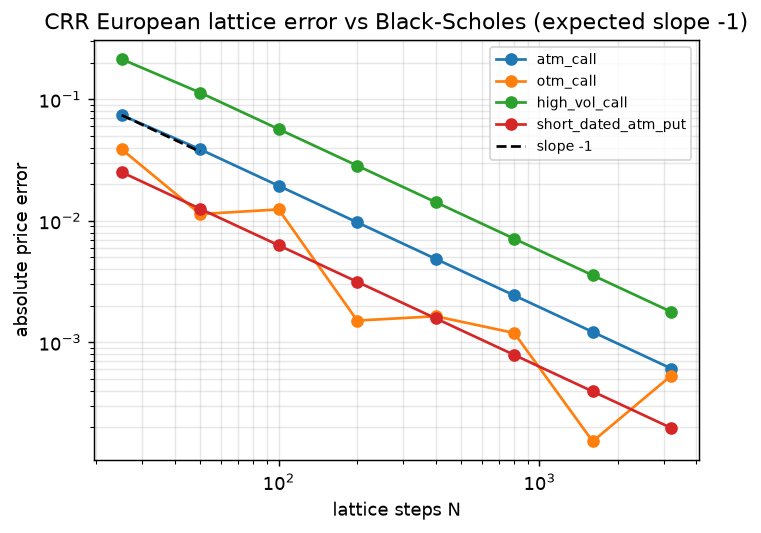
\includegraphics[width=0.72\textwidth]{experiments/pricing_validation/results/lattice_convergence.png}
\caption[Lattice convergence fitted on log-log axes]{CRR lattice error against $N$ on log-log
axes, the source of Table \ref{tab:crr-slopes}. Generated figure, committed at
\src{experiments/pricing_validation/results/lattice\_convergence.png}.}
\label{fig:crr}
\end{figure}

Comparing two different lattices is a different exercise and is treated as one. Against
QuantLib's \code{BinomialVanillaEngine(..., "crr", N)} --- a different discretisation of the
same dynamics --- the absolute gap in the extreme corners of the grid reaches
$1.82$ at 50 steps, $0.457$ at 200 steps and $0.114$ at 800 steps
(\src{benchmarks/quantlib/results/pricing_vs_quantlib.json}, \code{worst_absolute_error}).
Those numbers are not errors of our implementation: at 100\% volatility over five years on a
coarse tree the gap is \emph{smaller than each lattice's own error against Black--Scholes}, so
the test asserts the normalised property rather than a raw threshold
(\src{docs/limitations.md}, item 12). The summary key
\code{lattice_error_ratio_*} is reported only as informative away from cancellation
points, where the observed ratio spans $1.2\times 10^{-8}$ to 766
(\src{docs/limitations.md}, item 13;
\src{benchmarks/quantlib/results/pricing_vs_quantlib.json}).

\subsection{Asian and barrier options, and where discretisation actually costs}
Arithmetic Asian options are priced by Monte Carlo with the geometric average of the
\emph{same} paths as control variate; geometric Asians are priced both by simulation and by
the closed form of Section \ref{sec:mathematics}; barriers are up-and-out and down-and-out
with discrete monitoring and the optional continuity correction. Table \ref{tab:pathdep}
collects the worst relative errors against four oracle families recorded in
\src{benchmarks/quantlib/results/path_dependent_vs_quantlib.json}, on 25 rows with
200{,}000 paths each.

\begin{table}[t]
\caption[Path-dependent pricing against live oracles]{Path-dependent pricing against live oracles. The two barrier rows are the same
estimator with and without the \citet{broadie1997continuity} correction, so their gap is the
monitoring bias itself. Source:
\src{benchmarks/quantlib/results/path_dependent_vs_quantlib.json}, key
\code{worst_relative_error}.}
\label{tab:pathdep}
\centering\small
\begin{tabular}{llr}
\toprule
Family & reference & worst rel.\ error \\
\midrule
\code{asian_geometric_closed_form} & QuantLib analytic & $5.55\times 10^{-4}$ \\
\code{asian_geometric_simulated} & QuantLib analytic & $2.30\times 10^{-3}$ \\
\code{barrier_discrete} & continuous analytic & $1.40\times 10^{-1}$ \\
\code{barrier_bgk_corrected} & continuous analytic & $1.00\times 10^{-2}$ \\
\code{heston_degenerate} ($\xi = 0$) & Black--Scholes & $2.09\times 10^{-3}$ \\
\code{heston_analytic} & \code{AnalyticHestonEngine} & $4.47\times 10^{-3}$ \\
\bottomrule
\end{tabular}
\end{table}

The $14.0\%$ on the raw discrete barrier is not a bug but the economics of discrete
monitoring: a barrier checked at $M$ dates can only be crossed at those dates, so the
knockout probability is lower and the option worth more than the same contract monitored
continuously, and the correction reduces the gap by roughly fourteenfold
(\src{docs/model_cards/path_dependent_options.md}; \src{docs/limitations.md}, item 23).
The correction is an $O(\sqrt{dt})$ asymptotic result for a single barrier on a lognormal
diffusion, not an exact treatment of continuous monitoring, and the monitoring grid is the
simulation grid, so \code{steps} cannot be refined for one purpose without the other
(\src{docs/limitations.md}, items 23--24). The residual $5.5\times 10^{-4}$ on the geometric
Asian closed form is calendar-day rounding of the fixing schedule, because fixing and
monitoring dates are year-fraction arithmetic with no business-day convention
(\src{docs/limitations.md}, item 22).

Two defects in this area were found only because an oracle was consulted, and both are
described in Section \ref{sec:validation}: the continuity correction was initially implemented
moving the effective barrier the wrong way, with a test that asserted the wrong inequality and
passed because the implementation shared the misconception; and a mismatched fixing schedule
between the benchmark and the closed form produced a spurious 12\% disagreement between two
correct formulas (\src{docs/phase_reports/phase-04-path-dependent-heston.md}~\S6).

\subsection{Heston simulation}
The scheme is full-truncation Euler: the diffusion coefficient of both equations uses
$\max(v,0)$ and the variance update is clamped, with correlated normals built as $Z_1$ and
$\rho Z_1 + \sqrt{1-\rho^2}\,Z_2'$ so one stream per path carries the correlation exactly. It
is not an exact simulation, and every result carries a \code{note}, the clamp count in
\code{negative_variances_clamped}, and a bias probe
(\code{heston_step_refinement_gap}) (\src{docs/model_cards/heston.md}). Validation here is
deliberately described as weaker than the Black--Scholes section, for a structural reason: the
oracle is QuantLib's semi-analytic engine, itself a numerical quadrature, so the measured
$4.5\times 10^{-3}$ combines our discretisation bias with the oracle's integration tolerance
(\src{docs/limitations.md}, item 25). The only exactness claimed is the $\xi = 0$ collapse to
Black--Scholes, measured at $2.1\times 10^{-3}$ at 200{,}000 paths over 250 steps and read as
within sampling error (\src{docs/model_cards/heston.md}). Supporting checks in the same card:
the risk-neutral martingale property $\mathbb{E}[S_T] = S e^{(r-q)T}$ inside four standard
errors; positivity of every terminal and variance value over 20{,}000 paths including a
Feller-violating parameter set; the sign of skew (an out-of-the-money put priced higher at
$\rho = -0.9$ than at $\rho = +0.9$); and step refinement with differences inside four
combined standard errors for 20, 80 and 320 steps. There are no Heston Greeks, no smile
calibration, and no path-dependent payoff under Heston
(\src{docs/limitations.md}, item 27).

% ===========================================================================
\section{Monte Carlo Methods}
\label{sec:montecarlo}
% ===========================================================================

The estimator is $V_0 = e^{-rT} \mathbb{E}^{\mathbb{Q}}[\text{payoff}(S_T)]$ with
$\widehat{V}_N = e^{-rT} N^{-1} \sum_i \text{payoff}_i$ and
$\operatorname{SE}(\widehat{V}_N) = s/\sqrt{N}$, $s$ the sample standard deviation of the
discounted payoffs (\src{docs/mathematical_specification.md}~\S5). The separation of bias from
sampling error is load-bearing here: a European payoff drawn from the exact terminal transition
has zero discretisation bias, so all error is sampling error, whereas path-dependent payoffs and
the Heston scheme carry both. Each estimate reports price, standard error, confidence interval,
path count, count of independent units, seed, sample variance, the fitted control-variate
coefficient and wall-clock runtime (\src{docs/phase_reports/phase-03-monte-carlo.md}).

\subsection{Convergence and standard-error calibration}
Theory predicts $\widehat V_N - V_0 = O(N^{-1/2})$, and the claim is tested as a fitted slope
of $\log|\text{error}|$ on $\log N$ over $10^3$ to $3\times 10^6$ paths. Three scenarios give
$-0.614 \pm 0.089$, $-0.585 \pm 0.096$ and $-0.507 \pm 0.118$ against the theoretical $-0.5$,
all within 1.3 standard errors (\src{experiments/monte_carlo_convergence/results/summary.json},
key \code{convergence_slope_fit}; \src{README.md}).

\begin{figure}[t]
\centering
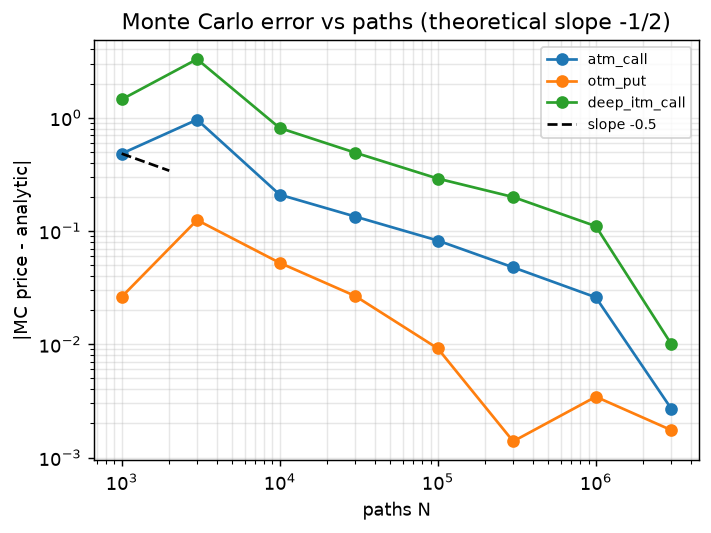
\includegraphics[width=0.72\textwidth]{experiments/monte_carlo_convergence/results/convergence_slope.png}
\caption[Fitted Monte Carlo convergence slope]{Fitted slope of $\log|\text{error}|$ on $\log N$
against the theoretical $-0.5$, the source of the figures in Section \ref{sec:montecarlo}.
Generated figure, committed at
\src{experiments/monte_carlo_convergence/results/convergence\_slope.png}.}
\label{fig:mc}
\end{figure}

A slope confirms the exponent; it does not confirm that the \emph{reported} standard error is
the right yardstick. Two further measurements address that. The first is coverage: over 12
combinations of seed count, path count and interval level, the empirical coverage of nominal
95\,\% and 99\,\% normal intervals fell inside the exact $\operatorname{Binomial}(n, level)$
band in 12 of 12 cases
(\src{experiments/monte_carlo_convergence/results/summary.json},
\code{coverage_intervals_inside_binomial_band}). The second is a z-score study: 492 rows
comparing our estimate against QuantLib's analytic price over 4 scenarios $\times$ 3 methods
$\times$ 40 seeds at 200{,}000 paths per run. With a correct estimator and a correctly
reported standard error, pooled z-scores should have mean near zero, standard deviation near
one, and about 95\,\% inside $\pm 2$; a systematically understated standard error shows up
first as a standard deviation well above one. The measured values in
Table \ref{tab:zscores} are consistent with all three
(\src{benchmarks/quantlib/results/monte_carlo_validation.json}).

\begin{table}[t]
\caption[Pooled z-scores of our Monte Carlo estimate against the live analytic oracle, 16]{Pooled z-scores of our Monte Carlo estimate against the live analytic oracle,
160 draws per method. Source:
\src{benchmarks/quantlib/results/monte_carlo_validation.json}, key
\code{z_score_vs_quantlib_analytic}.}
\label{tab:zscores}
\centering\small
\begin{tabular}{lrrrrr}
\toprule
Method & $n$ & mean & std & range & within $2$ SE \\
\midrule
antithetic & 160 & $-0.023$ & 1.014 & $-2.04$ to $+2.06$ & 98.8\,\% \\
control variate & 160 & $+0.050$ & 0.923 & $-2.11$ to $+1.78$ & 98.1\,\% \\
plain & 160 & $+0.031$ & 0.930 & $-2.40$ to $+2.10$ & 96.2\,\% \\
\bottomrule
\end{tabular}
\end{table}

One negative result is recorded rather than dropped: QuantLib's own Monte Carlo engine could
not be constructed in this build --- \code{MCEuropeanEngine} rejected every traits string
through the installed SWIG bindings --- so the artifact carries
\code{quantlib_mc_engine_used: false} with the reason, and the independent yardsticks that
\emph{are} used are the analytic price (the exact limit) and a NumPy/PCG64 simulation
(\src{benchmarks/quantlib/results/monte_carlo_validation.json};
\src{docs/limitations.md}, item 20).

\subsection{Variance reduction, measured out of sample}
Antithetic pairs share one normal $Z$ with the drift not negated, and satisfy the exactness
identity $S^{+} S^{-} = S^2 \exp[2(r - q - \sigma^2/2)T]$ to $10^{-12}$ relative. Control
variates use the geometric Asian average for arithmetic Asian payoffs, and an in-sample
adaptive coefficient. Because that coefficient is fitted on the same sample it is used to
reduce, the engine's own reported variance is mildly optimistic, and the project's answer is
to measure realised mean squared error out of sample over seed ensembles rather than to quote
the in-sample number (\src{docs/limitations.md}, item 19). Over 40 seeds $\times$ 3 path
budgets $\times$ 4 scenarios, the realised out-of-sample MSE reduction relative to plain
Monte Carlo ranges from $1.12\times$ to $2.77\times$ for antithetic sampling and from
$1.93\times$ to $40.47\times$ for control variates, with the largest gain on the
deep-in-the-money long-maturity call and the smallest on the short-dated out-of-the-money call
(\src{experiments/variance_reduction/results/summary.json}, key
\code{mse_reduction_vs_plain}; \src{docs/phase_reports/phase-03-monte-carlo.md}).

Two Level-1 identities guard against a variance-reduction estimator that is merely
\emph{popular}: a payoff affine in the control must reproduce the analytic price exactly, and
a constant payoff must return the discount factor. The deep-in-the-money call with strike 1.0
is affine in the control, and the control-variate estimator returns the analytic price to
about $10^{-12}$ with a standard error below $10^{-10}$ and fitted coefficient of 1
(\src{docs/phase_reports/phase-03-monte-carlo.md}~\S6;
\src{docs/model_cards/monte_carlo_gbm.md}). No quasi-Monte Carlo, Brownian bridge,
stratification or moment matching is implemented, and the engine is single-threaded
(\src{docs/limitations.md}, item 16).

% ===========================================================================
\section{Market Risk Estimation}
\label{sec:risk}
% ===========================================================================

Six point estimators, two bootstrap designs and three coverage tests were implemented in
Phase 5, and the phase's research question was statistical rather than numerical: are the
estimators and tests valid on synthetic distributions whose truth is known
(\src{docs/phase_reports/phase-05-market-risk.md}). The design of that experiment is worth
describing before its results, since it is what licenses the interpretations below. Data are
generated as Gaussian with $\sigma = 2\%$, a Student-$t$ with 3 degrees of freedom scaled to
the same unconditional standard deviation, and a GARCH(1,1) process with $\alpha = 0.10$,
$\beta = 0.85$ and $\omega$ chosen to match the same unconditional standard deviation
\citep{bollerslev1986generalized}; a fourth arm generates clustered violations from a
two-state Markov chain with stationary rate 5\,\% and $\Pr(\text{violate} \mid \text{violated})
= 0.25$, so the unconditional count is on target while the timing is clustered. Estimator
bias uses 400 replications; realised violation rates use 200 independent calibration blocks of
10{,}000 observations scored over 20{,}000 out-of-sample days each; coverage-test size uses
2{,}000 replications of 250 days; bootstrap coverage uses 400 replications at $n = 500$ with
1{,}500 resamples against an unconditional target computed from 2{,}000{,}000 draws. All
streams are seeded (\code{estimator 7000+r}, \code{backtest 100000+r}, and so on) so reruns
reproduce bit for bit (\src{experiments/var_backtesting/results/var_backtesting_validation.json}).

\subsection{Point estimators against known population values}
Table \ref{tab:var} reports the outcome that the layer is most careful about: the Gaussian fit
on fat-tailed data is wrong in \emph{opposite directions} at the two confidence levels,
because normal and $t$ quantile spacings differ. The empirical estimator tracks nominal at
both levels.

\begin{table}[t]
\caption[Out-of-sample realised violation rates (200 blocks $\times$ 20{,}000 days) again]{Out-of-sample realised violation rates (200 blocks $\times$ 20{,}000 days) against
population VaR levels. Read the two $t(3)$ rows together: a normal fit is not conservatively
wrong, it is wrong in opposite directions. Source:
\src{experiments/var_backtesting/results/estimator_convergence.csv}, block
\code{A_out_of_sample}; headline values also in \src{README.md}.}
\label{tab:var}
\centering\small\setlength{\tabcolsep}{4pt}
\begin{tabular}{llrrrr}
\toprule
Data & Level & Population VaR & nominal rate & empirical realised & Gaussian realised \\
\midrule
Gaussian $\sigma=2\%$ & 95\,\% & 0.03290 & 5\,\% & 5.034\,\% & 5.021\,\% \\
Gaussian $\sigma=2\%$ & 99\,\% & 0.04653 & 1\,\% & 1.014\,\% & 1.009\,\% \\
$t(3)$, same $\sigma$ & 95\,\% & 0.02717 & 5\,\% & 5.014\,\% & $\mathbf{3.291\,\%}$ \\
$t(3)$, same $\sigma$ & 99\,\% & 0.05243 & 1\,\% & 1.021\,\% & $\mathbf{1.389\,\%}$ \\
\bottomrule
\end{tabular}
\end{table}

At $n = 250$ on Gaussian data the bias of the Gaussian estimator at 95\,\% is
$-8.2\times 10^{-5}$, or $0.25\%$ relative
(\src{experiments/var_backtesting/results/var_backtesting_validation.json},
\code{headline.gaussian_95_var_bias_at_n250}). The layer's own reading of the two
$t(3)$ rows is that any explanation promising a one-sided safety margin from a normal fit is
false (\src{docs/model_cards/var_es.md}), and the estimators are retained as the reference
case, not as a defensible production choice (\src{docs/limitations.md}, item 30). Empirical
99\,\% VaR at 250 observations averages two or three order statistics, and
\code{quantile_standard_error} returns NaN rather than a plausible zero when the loss
distribution has a flat spot at that level --- common for option P\&L, where most paths finish
worthless (\src{docs/limitations.md}, item 29).

\subsection{Coverage tests: size, power and what each can see}
Table \ref{tab:kupiec} gives the four calibration arms. Three readings matter. First, the Kupiec test has
its nominal size --- $5.05\%$ rejection at the 5\,\% level, with exact binomial interval
$[4.13\%, 6.10\%]$ --- and is conservative at a 1\,\% cutoff ($0.0075$) because the statistic
is a function of an integer count. Second, power against an under-set level reaches 1.000 by
500 days. Third, and most useful: with clustered violations at the \emph{correct} marginal
frequency, Kupiec rejects $12.0\%$ of samples while the independence test rejects $55.4\%$,
and the converse holds too --- with a pure frequency error the independence test rejects only
$5$ to $6.8\%$ of the time, so it is not manufacturing a clustering signal
(\src{experiments/var_backtesting/results/coverage_test_size_power.csv};
\src{docs/phase_reports/phase-05-market-risk.md}~\S6).

\begin{table}[t]
\caption[Rejection rates of the three coverage statistics, 2{,}000 replications of 250 da]{Rejection rates of the three coverage statistics, 2{,}000 replications of 250 days at
a 5\,\% nominal cutoff. The last row is the discriminating result: an unconditional-frequency
test accepts a clustered model most of the time. Source:
\src{experiments/var_backtesting/results/coverage_test_size_power.csv}, block
\code{B_size_power}.}
\label{tab:kupiec}
\centering\small
\begin{tabular}{lrrr}
\toprule
Arm (true violation rate) & Kupiec & Independence & Conditional \\
\midrule
correctly calibrated iid ($0.05$) & 0.0505 & 0.0235 & 0.0380 \\
over-calibrated iid ($0.02$) & 0.7525 & 0.0206 & 0.6136 \\
under-set VaR ($0.12$) & 0.9860 & 0.0600 & 0.9620 \\
clustered, correct marginal ($0.05$) & 0.1200 & 0.5540 & 0.5345 \\
\bottomrule
\end{tabular}
\end{table}

These tests are marginal-frequency tests on a \emph{given} VaR series. They cannot validate
the model that produced the series, they have no power against an error that preserves both
the violation rate and its timing, and no multiple-comparison correction is applied across the
three statistics (\src{docs/limitations.md}, item 34). The implementation reports a
\code{degenerate} flag and NaN rather than a p-value of 1 when a state has no transitions, so
that a null result cannot be read as a clean bill of health (\src{docs/model_cards/var_es.md}).

\subsection{Uncertainty by resampling}
Percentile bootstrap intervals for the 95\,\% VaR, at a nominal 90\,\% level, $n = 500$,
400 replications, are given in Table \ref{tab:bootstrap}. On iid data the percentile interval
is slightly under nominal and the block design costs nothing. Under GARCH clustering the iid
design loses almost 28 percentage points of coverage; the block design recovers about 7 of
them, and the exact intervals do not overlap, so the improvement is real --- and the block
design still falls roughly 21 points short of nominal
(\src{experiments/var_backtesting/results/bootstrap_coverage.csv};
\src{docs/limitations.md}, items 31--32). This is reported as a limitation rather than fixed
by tuning the block length, and the default $\operatorname{round}(n^{1/3})$ rule is explicitly
flagged as a general-purpose choice that was never swept against coverage
(\src{docs/phase_reports/phase-05-market-risk.md}~\S8).

\begin{table}[t]
\caption[Bootstrap coverage of the true unconditional VaR]{Bootstrap coverage of the true unconditional VaR. Nominal level 90\,\%; intervals are
exact binomial. Source: \src{experiments/var_backtesting/results/bootstrap_coverage.csv}.}
\label{tab:bootstrap}
\centering\small
\begin{tabular}{llrl}
\toprule
Data & Design (block length) & Coverage & 95\,\% interval \\
\midrule
iid Gaussian & iid & 0.8725 & [0.8358, 0.9036] \\
iid Gaussian & moving block (8) & 0.8700 & [0.8330, 0.9014] \\
GARCH(1,1) clustered & iid & 0.6250 & [0.5755, 0.6726] \\
GARCH(1,1) clustered & moving block (8) & 0.6925 & [0.6447, 0.7374] \\
\bottomrule
\end{tabular}
\end{table}

No Cornish--Fisher expansion, extreme-value tail fit, filtered historical simulation or
expected-shortfall backtest of the Bellini--Frittelli or Acerbi--Tasche style named in the
register is implemented, and the estimand here is the unconditional quantile, not a
daily re-estimated conditional one (\src{docs/limitations.md}, items 33, 35).

% ===========================================================================
\section{Portfolio Optimization}
\label{sec:portfolio}
% ===========================================================================

The portfolio layer contains three covariance estimators and five solvers, 2{,}695 lines
of header and source across the layer including bindings
(\src{docs/phase_reports/phase-06-portfolio-optimisation.md}~\S3). Two properties distinguish
it from a typical implementation exercise.

The first is that \emph{every solution carries a certificate}. The active-set solver treats
each candidate support as a saddle-point KKT system rather than forming $\Sigma^{-1}$, and
verifies the answer against the original data for primal feasibility, dual feasibility and
complementary slackness; \code{verified_optimal} is therefore a proof, not a convergence
message (\src{docs/model_cards/portfolio_covariance_and_optimisation.md}). The choice is
load-bearing: with a flat or duplicated asset, the normal equations return the
minimum-\emph{norm} stationary point rather than the optimum --- on $\Sigma =
\operatorname{diag}(0.04, 0)$ they put the whole position in the risky asset and report
variance 0.04, where the saddle system returns the true answer of holding the flat asset at
zero variance, and that case is a test rather than a footnote. Likewise, ill-conditioned
inputs are refused rather than repaired: the guarded \code{LLT} solve returns NaN with a
reason when the matrix is not positive definite or when $\operatorname{rcond} < 10^{-12}$,
and every estimate carries its spectrum, \code{positive_semidefinite} flag and note
(\src{docs/model_cards/portfolio_covariance_and_optimisation.md}).

The second is that the layer's headline result is about the \emph{input}, not the solver.

\subsection{Agreement with independent solvers}
Table \ref{tab:optimisers} reports the 75-problem benchmark (5 asset counts $\times$ 3 seeds
$\times$ 5 problem families) against PyPortfolioOpt's SLSQP route and cvxpy with OSQP for the
quadratic programmes and SCS for the conic ones. Weights and objectives are reported
separately and deliberately, because on degenerate problems they carry different meanings: an
LP optimum may be an entire face, so the vertex each method reports is a property of the
algorithm, while the objective is the comparable quantity
(\src{docs/model_cards/portfolio_covariance_and_optimisation.md}).

\begin{table}[t]
\caption[Level-2 agreement on 75 problems]{Level-2 agreement on 75 problems. ``Weights'' is the largest coordinate difference
against the named oracle; ``objective'' is the largest relative gap in the optimised
quantity. Risk parity has no PyPortfolioOpt implementation in version 1.6.0 and CVaR is
solved by PyPortfolioOpt through cvxpy, so those columns are labelled duplicates rather than
two independent references. Source:
\src{benchmarks/pyportfolioopt/results/optimisation_vs_oracles.json}, key
\code{agreement.per_problem}.}
\label{tab:optimisers}
\centering\small\setlength{\tabcolsep}{4pt}
\begin{tabular}{lrrr}
\toprule
Problem & weights vs PyPortfolioOpt & weights vs cvxpy & worst relative objective gap \\
\midrule
\code{min_variance} & $3.5\times 10^{-13}$ & $2.4\times 10^{-12}$ & $7.3\times 10^{-16}$ \\
\code{efficient_return} & $4.0\times 10^{-13}$ & $2.4\times 10^{-12}$ & $6.5\times 10^{-14}$ \\
\code{max_sharpe} & $7.0\times 10^{-9}$ & $7.0\times 10^{-9}$ & $1.2\times 10^{-11}$ \\
\code{risk_parity} & $1.4\times 10^{-11}$ & $1.4\times 10^{-11}$ & $2.8\times 10^{-12}$ \\
\code{minimise_cvar} & $4.7\times 10^{-7}$ & $4.7\times 10^{-7}$ & $4.5\times 10^{-9}$ \\
\bottomrule
\end{tabular}
\end{table}

Constraints were checked on all 75 solutions independently of the agreement figures: the worst
budget residual is $1.4\times 10^{-12}$ and the worst long-only violation is exactly 0
(\src{benchmarks/pyportfolioopt/results/optimisation_vs_oracles.json};
\src{README.md}). The estimators themselves were compared separately, in tests rather than in
the benchmark: sample covariance agrees with \code{numpy.cov(ddof=1)} to
$7.2\times 10^{-16}$ relative, and the Ledoit--Wolf shrinkage estimate agrees with
scikit-learn's \code{LedoitWolf} to $7\times 10^{-19}$ absolute
(\src{tests/python/test_covariance_vs_oracles.py}; \src{README.md}).

Two findings in this comparison came from checking, not from assuming, and both are recorded
in Section \ref{sec:validation}: the first draft of the benchmark measured the rounding of
PyPortfolioOpt's \code{clean_weights()} rather than the optimisation, and the max-Sharpe row
is loose on our side --- both oracles agree with each other to about $10^{-10}$ while each
sits at $7\times 10^{-9}$ from us, which a full-precision in-process probe resolved by showing
the achieved Sharpe ratio matching to $\le 1.3\times 10^{-12}$ absolute, so the weight gap is
the flat frontier rather than a wrong answer
(\src{docs/phase_reports/phase-06-portfolio-optimisation.md}~\S6).

\subsection{What estimating a covariance costs}
Numerical agreement of order $10^{-9}$ is not the interesting quantity, because the matrix
being inverted is an estimate. A rolling-origin study on a synthetic two-regime factor
process --- 8 assets, 600 monthly observations, a regime break at observation 300 where both
factor volatilities double and loadings shift by 0.35, a 20-day forward horizon stepped by 5,
EWMA $\lambda = 0.94$ --- scores 1{,}119 frozen portfolios against a forward covariance known
in closed form, over 373 solved windows, and reports the ratio of each frozen portfolio's
forward variance to that of the portfolio an informed solver would have held
(\src{experiments/portfolio_optimization/results/portfolio_optimisation_study.json},
key \code{data}). Table \ref{tab:cost} gives the result.

\begin{table}[t]
\caption[Forward variance ratio against an informed solver, by estimation window and esti]{Forward variance ratio against an informed solver, by estimation window and
estimator. Values above 1 mean the estimated matrix costs extra variance. Source:
\src{experiments/portfolio_optimization/results/portfolio_optimisation_study.json}, key
\code{estimation_cost.by_window_and_estimator}.}
\label{tab:cost}
\centering\small
\begin{tabular}{lrrr}
\toprule
Window & sample & EWMA & shrinkage \\
\midrule
40 & 1.2176 & 1.2560 & \textbf{1.1686} \\
60 & 1.1626 & 1.2287 & \textbf{1.1463} \\
125 & \textbf{1.1326} & 1.2334 & 1.1331 \\
250 & 1.2194 & 1.2453 & 1.2265 \\
\bottomrule
\end{tabular}
\end{table}

\begin{figure}[t]
\centering
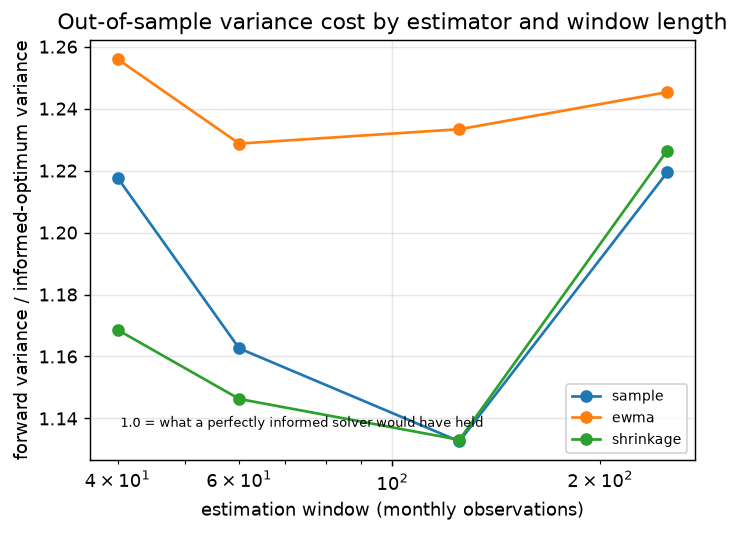
\includegraphics[width=0.74\textwidth]{experiments/portfolio_optimization/results/estimator_cost_by_window.png}
\caption[Forward variance cost by estimation window and estimator]{Forward variance ratio against
an informed solver by window and estimator, the source of Table \ref{tab:cost}. Generated figure,
committed at \src{experiments/portfolio\_optimization/results/estimator\_cost\_by\_window.png}.}
\label{fig:cost}
\end{figure}

Six readings come out of this artifact, each quoted with the figure that supports it.
(a) Estimation, not optimisation, is the dominant error: the smallest measured penalty is
about $13\%$ in forward variance (best cell $1.1326$) against a worst numerical objective
disagreement of $4.5\times 10^{-9}$, roughly seven and a half orders of magnitude
(\src{experiments/portfolio_optimization/results/portfolio_optimisation_study.json},
\code{findings.estimation_is_the_dominant_cost}). (b) Shrinkage wins where instability
bites: at window 40 it lowers the ratio from $1.2176$ to $1.1686$, cuts turnover from $0.2067$
to $0.1381$, and raises effective asset count from $5.10$ to $5.97$. (c) More history is not
monotonically better: window 250 is $0.087$ \emph{worse} than 125 for the sample estimator,
because it pools two different joint distributions. (d) Non-stationarity dominates estimation
error: forward slices straddling the regime break cost $1.57$ to $1.60$ for every estimator,
against $1.075$ to $1.222$ inside a single regime. (e) The refusal is the point: on a
5-observation window of 8 assets the sample matrix has condition number $6.7\times 10^{17}$
and the solve refuses, while the shrunk matrix at condition number $8.0$ solves and costs
$0.0086$ rather than $0.0111$ in forward volatility. (f) An optimiser is only as honest as its
input: with an asset flat in the sample but volatile in the truth, the solver correctly
concentrates into it ($\text{effective\_assets} = 1.00$) and carries $3.5\times$ the forward
volatility of the well-conditioned case.

A fourth objective's behaviour completes the argument. Comparing all four objectives fitted on
the same shrinkage-estimated windows and scored on the same forward slice, max-Sharpe --- the
only one that consumes an estimated \emph{mean} --- is worst on every forward metric, with
forward volatility $0.01856$ against $0.01166$ for minimum variance and realised worst loss
$0.02691$ against $0.01441$
(\src{experiments/portfolio_optimization/results/objective_comparison.csv};
\src{experiments/portfolio_optimization/results/portfolio_optimisation_study.json},
key \code{objective_comparison}). This is error maximisation measured rather than asserted,
and it is why the project records that no expected-return model exists in this codebase and
that any use treating a sample mean as skill inherits the consequence
(\src{docs/limitations.md}, item 37).

Robustness cases were run alongside: near-collinear twins give condition numbers of
$4.2\times 10^{8}$ (sample) and $6.3\times 10^{8}$ (EWMA), with the solve still succeeding and
the estimate's note reporting the instability, against $56.9$ for the shrunk matrix on the same
input (\src{experiments/portfolio_optimization/results/solver_robustness.csv}). With every asset
below the risk-free rate the maximum Sharpe ratio is negative and attained at a corner rather
than a tangency, and the search certifies the least-bad portfolio; with an unreachable target the
solution reports \code{feasible = false} with the size of the bound violation and a note naming
the violated bounds, because such a target still has an equality solution --- it simply requires
shorting (\src{docs/model_cards/portfolio_covariance_and_optimisation.md}).

The scope is narrow and stated as such: long-only, fully invested, single-period, with no
position caps, sector or turnover constraints, no transaction cost netted against return, an
EWMA filtered about zero, and a shrinkage target of the scaled identity rather than a diagonal
or custom target (\src{docs/limitations.md}, items 36--40). The simplex is dense, two-phase,
uses Bland's rule, and is exponential in the worst case; it was validated at $\le 12$ assets
and 250 scenarios and is not a production LP (\src{docs/limitations.md}, item 41).

% ===========================================================================
\section{Stress Testing}
\label{sec:stress}
% ===========================================================================

The stress layer, 1{,}152 lines across four headers and four sources, answers a different
question from the pricing or optimisation code: given a book described by factor exposures
and a scenario described as data, what happens to the risk, and can the answer be attributed
to its causes (\src{docs/phase_reports/phase-07-stress-testing.md}~\S1)? It maps exposures
and never re-prices instruments. The mapping is deterministic,
\begin{equation}
\Delta \text{P\&L} = \sum_i \delta_i s_i + \gamma_i s_i^2 + d_i a_i + v_i a_i + c_i a,
\end{equation}
where $\gamma$ is quoted with the one-half absorbed --- stated because the Black--Scholes gamma
a caller would derive it from does not carry it, and the revaluation test depends on the
convention. Portfolio dispersion uses the first-order beta $\delta + \text{duration} +
\text{vega} + \text{credit}$, because convexity moves the mean rather than the variance and
folding a squared term into a covariance would make the second moment depend on the scenario's
direction (\src{docs/phase_reports/phase-07-stress-testing.md}~\S2).

Factor classes decide what a shock means: equity factors are shocked relatively, rate,
volatility and credit factors absolutely, both units are resolved wherever the quoted level
permits, and a shock that states both and disagrees is rejected. A distinction that survives
aggregation is that an absent sensitivity is not a zero: an empty \code{vega} block means no
vega sensitivity was recorded, which is a weaker and more honest claim than vega being zero,
and it is what forces \code{beta_of} to take the factor count rather than sizing itself from
whichever block happens to be first (\src{docs/model_cards/scenario_stress_testing.md};
\srcin{cpp/src/stress/engine.cpp}).

\begin{figure}[t]
\centering
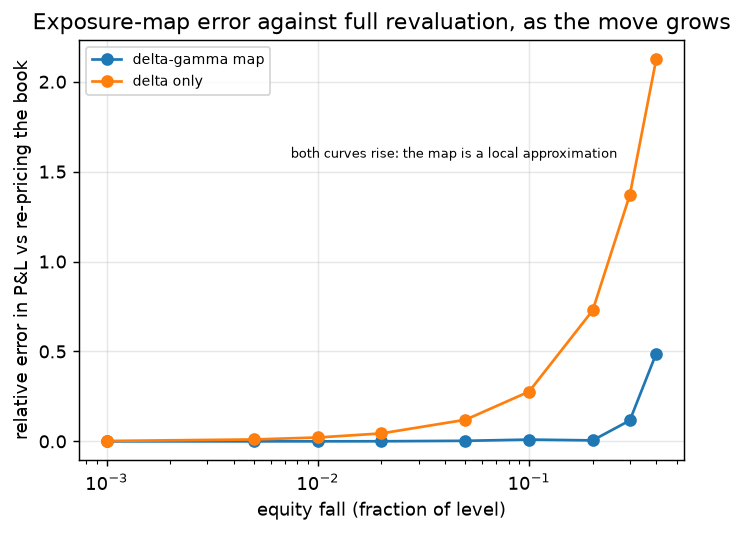
\includegraphics[width=0.72\textwidth]{experiments/stress_testing/results/linearisation_error.png}
\caption[Measured truncation error of the exposure map]{Relative P\&L error of the delta--gamma
and delta-only maps against a full Black--Scholes revaluation, the source of
Table \ref{tab:linear}; the non-monotone segment is visible. Generated figure, committed at
\src{experiments/stress\_testing/results/linearisation\_error.png}.}
\label{fig:lin}
\end{figure}

\subsection{Closure, independent numerics, and the measured truncation error}
Attribution is exact by construction, so its residuals are a bug report rather than a
tolerance. Across 28 scenario/book combinations the worst factor-attribution residual,
position-attribution residual and level/dispersion decomposition residual are each exactly
$0.0$ (\src{experiments/stress_testing/results/stress_testing_study.json}, key
\code{attribution_closure}; \src{experiments/stress_testing/results/scenario_ranking.csv}).
The level/dispersion split of $\Delta\text{VaR}$ is exact only because the Gaussian quantile is
affine in (mean, sigma); the code comment says so, and the limitation says the split would not
telescope for a historical or Cornish--Fisher estimator (\src{docs/limitations.md}, item 45).
Independent recomputation in NumPy of the mapping, covariance shift, historical replay and its
quantile agrees to $10^{-9}$ relative, stressed VaR against SciPy's own normal quantile to
$10^{-9}$, and Euler component VaR against a central-difference gradient of the VaR formula to
$3\times 10^{-10}$ against a bound set at $10^{-6}$ --- about 3{,}000-fold inside its
tolerance, which is what makes the check discriminate rather than accommodate
(\src{tests/python/test_stress_vs_oracles.py};
\src{docs/phase_reports/phase-07-stress-testing.md}~\S6).

The linearisation error is then measured against the thing it replaces: a three-strike call
book shocked through the exposure map and re-priced through the Phase 2 Black--Scholes engine.

\begin{table}[t]
\caption[Truncation error of the exposure map against a full Black--Scholes revaluation o]{Truncation error of the exposure map against a full Black--Scholes revaluation of the
same book, as relative error in P\&L. The delta--gamma column is \emph{not} monotone in the
size of the move, which is why no single validity range is claimed. Source:
\src{experiments/stress_testing/results/linearisation_error.csv};
\src{experiments/stress_testing/results/stress_testing_study.json}, key
\code{linearisation}.}
\label{tab:linear}
\centering\small
\begin{tabular}{lrr}
\toprule
Equity fall & delta--gamma rel.\ error & delta only rel.\ error \\
\midrule
0.1\,\% & $1.35\times 10^{-6}$ & $2.10\times 10^{-3}$ \\
0.5\,\% & $3.36\times 10^{-5}$ & $1.06\times 10^{-2}$ \\
1\,\%   & $1.33\times 10^{-4}$ & $2.15\times 10^{-2}$ \\
2\,\%   & $5.22\times 10^{-4}$ & $4.42\times 10^{-2}$ \\
5\,\%   & $3.02\times 10^{-3}$ & $1.20\times 10^{-1}$ \\
10\,\%  & $9.75\times 10^{-3}$ & $2.77\times 10^{-1}$ \\
20\,\%  & $5.37\times 10^{-3}$ & $7.28\times 10^{-1}$ \\
30\,\%  & $1.16\times 10^{-1}$ & $1.37$ \\
40\,\%  & $4.88\times 10^{-1}$ & $2.13$ \\
\bottomrule
\end{tabular}
\end{table}

Convexity buys two orders of magnitude at a 1\,\% move, and the delta-only map is already wrong
by more than a fifth of the P\&L there. Between 10\,\% and 20\,\% the delta--gamma error
\emph{improves}, because the cubic term changes sign through the strike region and partially
cancels; the project's reading is that a bound read off one point of this curve would be wrong
at another (\src{docs/limitations.md}, item 43). Monte Carlo stress VaR at 400{,}000 paths
reproduces the parametric number within 1\,\%, with the longer run the closer one, and the
sampler's realised dispersion recovers the supplied covariance to within 2\,\%, cross-checked
against NumPy's generator --- a different RNG and a different normal transform, so a
reproducibility defect in our path could not agree with it by construction
(\src{docs/phase_reports/phase-07-stress-testing.md}~\S6).

\subsection{The finding: stress inverts the safety ranking}
Four books were built by the Phase 6 optimisers --- equal weight, minimum variance, risk
parity, minimum CVaR --- on a synthetic 10-factor fixture (six equities, one rate, one
volatility, one credit spread) with notionals of 100{,}000{,}000 and 95\,\% confidence, then
ranked by base parametric VaR and re-ranked under each of seven named scenarios. Table
\ref{tab:ranking} summarises.

\begin{table}[t]
\caption[VaR multipliers by scenario, and how many of the four books change rank]{VaR multipliers by scenario, and how many of the four books change rank.
``Level rank'' is the absolute risk ranking by stressed VaR; ``sensitivity rank'' is the
ranking by multiplier. Source:
\src{experiments/stress_testing/results/stress_testing_study.json}, key \code{ranking}.}
\label{tab:ranking}
\centering\small\setlength{\tabcolsep}{4pt}
\begin{tabular}{lrrrrl}
\toprule
Scenario & max mult. & min mult. & spread & rank kept & most sensitive \\
\midrule
\code{equity_-20pct} & 6.113 & 5.234 & 0.168 & 0 of 4 & \code{min_variance} \\
\code{risk_off} & 5.606 & 4.934 & 0.136 & 0 of 4 & \code{min_variance} \\
\code{vol_x2} & 2.000 & 2.000 & 0.000 & 0 of 4 & all equal \\
\code{correlation_+0.2} & 1.367 & 1.297 & 0.054 & 0 of 4 & \code{risk_parity} \\
\code{rates_+200bp} & 1.010 & 1.005 & 0.005 & 0 of 4 & \code{risk_parity} \\
\code{credit_+150bp} & 1.0004 & 1.0002 & 0.0002 & 0 of 4 & \code{risk_parity} \\
\code{rates_-100bp} & 0.998 & 0.995 & 0.002 & 0 of 4 & \code{min_cvar} \\
\bottomrule
\end{tabular}
\end{table}

No book changes its absolute risk rank in any of the seven scenarios, and the report is careful
to say why that is not reassuring: the books started $20.8\%$ apart in base VaR
($\text{base\_var\_spread} = 0.2077$) while the largest stress-induced multiplier spread was
$16.8\%$, so the stability is a near miss rather than a property of the optimisers
(\src{docs/limitations.md}, item 48). Ranked by multiplier instead of by level, the order
inverts: under the equity crash all four books change rank, and \code{min_variance}, the
safest book under normal dispersion, is the most stress-sensitive at $6.11\times$, while
\code{equal_weight}, the riskiest normally, is the least at $5.23\times$
(\src{experiments/stress_testing/results/stress_testing_study.json}; \src{README.md}). This
is the Phase 6 result seen from the other end: optimising for an estimated covariance
concentrates a book, and concentration is exactly what an equity stress amplifies. The
\code{vol_x2} scenario gives every book a multiplier of exactly 2.000 with zero spread and a
level share of exactly 0.0 --- all of its VaR increase is dispersion, none of it loss already
taken --- which is the decomposition working as designed.

Beyond this, three scenario kinds exist (deterministic, historical replay, Monte Carlo);
\code{assumptions} is a required field the engine reads and echoes, so a scenario cannot present
a number without provenance; and a single-scenario result returns NaN for VaR and ES rather than
relabelling one outcome as a risk measure (\src{docs/model_cards/scenario_stress_testing.md}).
Missing capabilities are listed rather than implied: no higher-order terms, Gaussian scenario
moves only, one factor per asset class so a rate shock is parallel by construction and a
butterfly or steepener is inexpressible, and no reverse stress testing --- the engine answers
``what does this shock do'' and not ``what shock would produce this loss'', which is the
direction most supervisory use of the word means (\src{docs/limitations.md}, items 44, 46, 47).

% ===========================================================================
\section{Numerical Validation}
\label{sec:validation}
% ===========================================================================

Validation is organised around three levels defined in \src{docs/validation_protocol.md} before
any code existed, and executed per phase with real output.

\begin{itemize}
\item \textbf{Level 1 --- analytical identity.} Parity identities, degenerate limits, $ud = 1$,
the no-early-exercise theorem, control-variate exactness on an affine payoff, the geometric-average
variance limit, constraint residuals that must vanish, and analytic Greeks against central
differences with a Richardson error estimate instead of a tuned tolerance.
\item \textbf{Level 2 --- live independent oracle.} QuantLib's analytic and lattice engines
\citep{quantlib}, SciPy \citep{scipy2020}, and for the portfolio layer PyPortfolioOpt (behind
SciPy's SLSQP) \citep{pyportfolioopt}, cvxpy with OSQP and SCS \citep{cvxpy}, and scikit-learn
\citep{sklearn2011}. Oracle versions and configuration are printed into each artifact; no oracle
output is pasted into a test.
\item \textbf{Level 3 --- statistical.} Convergence order fitted on log-log axes with standard
errors; interval coverage against the exact binomial band; size and power of coverage tests;
rolling-origin portfolio cost measured against a forward covariance known in closed form.
\end{itemize}

\subsection{How tolerances are set}
Both absolute and relative error are reported for every comparison, and tiers follow the source
of the bound: deterministic analytic checks are tight, pinned in the Phase 2 test files and
justified by double rounding rather than trial and error; lattice and Monte Carlo bounds are
looser and justified by theory; statistical checks are hypothesis-test based (coverage within a
binomial interval, backtest p-values, slope tolerance bands)
(\src{docs/validation_protocol.md}~\S2). Two prohibitions do most of the work: lowering a
tolerance or deleting a failing test to make CI green is forbidden, and expected values must be
\emph{derived}, never transcribed.

The derived-values rule was earned. Phase 5 caught two invented constants in its own tests: a
chi-square 5\,\% point for 4 degrees of freedom filed under 5 degrees of freedom, and a tail
probability that contradicted the closed form $\exp(-x/2)$ for 2 degrees of freedom. Both
looked plausible; both were wrong. Critical values are now solved by \code{chi_square_isf}
from the same survival function that produces the p-value, so a statistic and its threshold
cannot drift apart by someone mistyping a table
(\src{docs/validation_protocol.md}~\S2; \src{docs/model_cards/var_es.md}).

\subsection{Validation matrix}
Table \ref{tab:matrix} is the Phase 10 matrix required by \src{PROJECT_SPEC.md}, organised by
the artifact a number came from. The project's own version of the same table, which adds the
bound each \emph{test} asserts next to the error actually measured and labels a bound chosen by
observation as \emph{(measured)}, is
\src{docs/validation_matrix.md}; its status vocabulary distinguishes \code{validated},
\code{validated (L1 only)}, \code{partially validated} and \code{weaker than claimed}. Status
values in Table \ref{tab:matrix} are the phase-gate verdicts recorded in the reports named there,
and no global test-coverage or pass-rate figure is asserted anywhere in this report beyond the
counts the phase reports themselves record.

Three rows of that matrix carry caveats that the table form flattens, and they are worth
restating. Rho's relative error of $1.07\times 10^{-7}$ occurs on values passing through zero,
where the absolute error is $5.12\times 10^{-13}$, which is why relative errors are reported only
above the floor the artifact records. The binomial row asserts a \emph{rate}, not a value: a
$1.82$ gap at 50 steps is the $O(dt)$ truncation the model card derives, and the falsifiable
claim is the fitted slope. And the stress engine's oracle bounds the arithmetic, not the scenario:
re-pricing the same book through Black--Scholes shows that the map is a correct second-order
expansion and how fast that stops being true, but it says nothing about whether a chosen
scenario is the right one to run, because there is no independent implementation of a management
assumption (\src{docs/validation_matrix.md}).

\begin{table}[p]
\caption[Validation matrix]{Validation matrix. ``Tolerance/bound'' is either the bound asserted in the named test
or the measured value where the artifact records one. Every row's evidence is a committed
artifact.}
\label{tab:matrix}
\centering\footnotesize
\begin{tabular}{@{}>{\raggedright\arraybackslash}p{2.9cm}>{\raggedright\arraybackslash}p{4.0cm}>{\raggedright\arraybackslash}p{2.5cm}>{\raggedright\arraybackslash}p{3.4cm}@{}}
\toprule
Component & Level and method & Oracle & Measured result \\
\midrule
Normal distribution, inverse, statistics & L1 identities; L2 dense grid & SciPy \citep{scipy2020} & max abs.\ err $< 10^{-12}$; L3 KS on 50{,}000 normals, $\chi^2$ on 80{,}000 uniforms \\
BS price \& Greeks & L1 parity and limits; L2 live repricing & QuantLib analytic & Tables \ref{tab:bs-agreement}; parity $7.99\times10^{-15}$ \\
CRR lattice & L1 $ud=1$, no-early-exercise; L2 lattice engine; L3 slope fit & QuantLib lattice engine & Table \ref{tab:crr-slopes}; corner gap read as normalised property \\
MC European & L1 exactness identities; L2 analytic limit; L3 slope \& coverage & QuantLib analytic + NumPy/PCG64 & Tables \ref{tab:zscores}; slopes $-0.61$ to $-0.51$; 12/12 coverage \\
Variance reduction & L3 out-of-sample MSE over seed ensembles & --- (own estimator) & $1.12$--$2.77\times$ antithetic, $1.93$--$40.47\times$ control variate \\
Asian (geometric) & L1 variance limit; L2 analytic & QuantLib & $5.5\times10^{-4}$ (day rounding) \\
Barrier & L2 continuous analytic; L3 monitoring refinement & QuantLib barrier engine & Table \ref{tab:pathdep} rows 3--4 \\
Heston & L1 $\xi=0$ collapse; L2 semi-analytic; L3 step refinement & QuantLib semi-analytic Heston engine & $2.1\times10^{-3}$ / $4.5\times10^{-3}$, weaker than BS by construction \\
VaR / ES estimators & L1 definition; L2 SciPy quantiles and quadrature; L3 realised rates & SciPy & Table \ref{tab:var} \\
Bootstrap intervals & L3 coverage vs exact binomial band & own exact intervals & Table \ref{tab:bootstrap} \\
Kupiec / Christoffersen & L3 size, power, discrimination & chi-square from own special functions & Table \ref{tab:kupiec} \\
Covariance estimators & L2 & \code{numpy.cov}, scikit-learn & $7.2\times10^{-16}$ rel; $7\times10^{-19}$ abs \\
Portfolio solvers & L1 certificates; L2 two solver families & PyPortfolioOpt, cvxpy & Table \ref{tab:optimisers} \\
Stress mapping \& attribution & L1 residuals; L2 NumPy/SciPy and full BS revaluation; L3 MC stress VaR & Black--Scholes engine, NumPy, SciPy & Tables \ref{tab:linear}, \ref{tab:ranking}; residuals $0.0$ \\
Python/C++ consistency & exact match against a compiled reference tool & own binary & \code{rel = 0, abs = 0} on 256 normals and more \\
Data layer & provenance integrity and refusal behaviour & live responses & 13/13 fixture digests match; socket-blocking test passes \\
\bottomrule
\end{tabular}
\end{table}

\subsection{Defects found by the process}
Reporting these is not an apology; it is the part of the evidence with the most information in
it. A validation regime that reported nothing across Phases 1 to 9 would more plausibly have
been measuring the wrong thing.

\paragraph{Lanczos denominator off by one.} In \srcin{cpp/src/math/special.cpp}, the series
denominator used $z + i - 1$ where the definition requires $z + i$. The symptom was
$\log\Gamma(13) = 20.078$ against 19.987, and \code{log_gamma(0.25)} returning NaN --- the log
of a negative sum. After correction the implementation agrees with \code{math.lgamma} to
$1.8\times 10^{-15}$ maximum absolute error
(\src{docs/phase_reports/phase-05-market-risk.md}~\S5).

\paragraph{A likelihood term that made a likelihood ratio negative.} The Kupiec statistic
dropped $x \ln p$ and used $x \ln x$ in \emph{both} likelihoods. The result reduced to its first
term and gave $-0.9989$ for 13 violations in 250 days --- a likelihood ratio cannot be
negative --- with the p-value pinned at 1.0, so a badly under-set VaR was reported as a pass.
Both binomial likelihoods were rewritten from the definition, and a $0 \log 0$ limit helper
replaces the term that hid the bug (\src{docs/phase_reports/phase-05-market-risk.md}~\S5).
This is arguably the most important defect in the project: it made a risk-model validation
test incapable of failing.

\paragraph{A quantile read from an unsorted array.} \code{monte_carlo_var} computed its
quantile from an unsorted loss array, reporting $-0.41$ for the VaR of a standard-normal
P\&L sample where the population value is about $1.64$; the confidence interval was computed
on the same garbage. The fix sorts first, and the \code{*_sorted} primitives now refuse
unsorted or NaN input rather than returning a plausible number
(\src{docs/phase_reports/phase-05-market-risk.md}~\S5).

\paragraph{Catastrophic cancellation in an incomplete gamma.} The lower regularised gamma was
computed as $1 - (1 - P)$, so $P(20, 0.01) = 4.07\times 10^{-59}$ came out as exactly 0.0. Both
tails are now evaluated from the representation that is not sitting at one
(\src{docs/phase_reports/phase-05-market-risk.md}~\S5).

\paragraph{Comparing against a rounded oracle output.} The first portfolio benchmark compared
weights against PyPortfolioOpt's \code{clean_weights()}, which rounds to five decimals and
zeroes anything under $10^{-4}$. That floored every disagreement at about $5\times 10^{-6}$, so
the test was measuring the oracle's rounding rather than the optimisation --- and the tests
carried the same defect behind a comment claiming $10^{-9}$ agreement while asserting
$5\times 10^{-5}$. Reading raw solver output tightened the quadratic comparisons by roughly
seven orders of magnitude (\src{docs/phase_reports/phase-06-portfolio-optimisation.md}~\S6).
A related trap in the same area: scikit-learn's \code{EmpiricalCovariance} is the biased
maximum-likelihood estimator with divisor $T$ while this project's is unbiased with $T-1$, so
comparing them returns about $6\times 10^{-6}$ on a 400-observation window --- a convention
difference that looks exactly like a bug. The reference has to be \code{numpy.cov(ddof=1)}, and
the test says so in its own name.

\paragraph{A continuity correction implemented backwards.} As described in
Section \ref{sec:pricing}, the barrier correction initially moved the effective barrier away
from the spot, and the test asserted the wrong inequality and passed, because the test shared
the misconception. The oracle comparison is what caught it; the tests now assert the tightened
barrier, the cheaper price and the reduced error
(\src{docs/model_cards/path_dependent_options.md};
\src{docs/phase_reports/phase-04-path-dependent-heston.md}).

\paragraph{An empty sensitivity vector sizing a beta.} The stress layer's portfolio beta was
once sized from whichever exposure block happened to be first. For a book whose only
sensitivity is vega, the \code{delta} vector is empty, and the beta came out empty --- which
allocated exactly zero risk to a position that carried real risk. The function now takes the
factor count, and the reason is recorded in the code comment and the model card
(\srcin{cpp/src/stress/engine.cpp}; \src{docs/model_cards/scenario_stress_testing.md}).

\paragraph{A test runner that hid unexecuted tests.} \code{ctest --preset dev} uses
\code{stopOnFailure: true}, and Phase 5's cases are numbered after the earlier ones, so a run
that halted printed ``99\,\% tests passed, 1 failed out of 94'' while 16 later cases had never
executed. Running the Catch2 binary directly exposed 6 failing cases and 11 failing assertions.
Every phase report from that point quotes the Catch2 case count and the CTest total together,
because the discrepancy is what to look for (\src{docs/phase_reports/phase-05-market-risk.md}
\S5, \S8).

\paragraph{Provenance that named the wrong commit.} \code{git_commit} was captured at
configure time, so every artifact from Phases 1--4 named the \emph{previous} phase's commit
while the working tree held the real change --- and a clean tree turned that into a confident
false statement. Artifacts now record run-time \code{git_commit}, \code{binary_git_commit},
\code{working_tree_dirty} and \code{uncommitted_paths}, plus a provenance sentence that
differs for the four reachable cases; \code{artifact_manifest} also stopped storing absolute
paths, which had been publishing a developer's home directory in committed evidence files
(\src{docs/validation_protocol.md}~\S3;
\src{docs/phase_reports/phase-05-market-risk.md}~\S5).

\paragraph{Two defects in the evidence tooling and one in the CLI.} A
\code{!!}-prefix check applied to the path instead of the status column was a dead branch
written from a wrong model of \code{git status --porcelain}, caught by the first tests written
for the parser (\src{docs/phase_reports/phase-05-market-risk.md}~\S5). The CLI's
analytic-versus-finite-difference check compared against a guessed $5\times 10^{-5}$ gap and
failed at $6.39\times 10^{-5}$, which is the correct truncation error; it was replaced by an
assertion about the ratio of successive gaps rather than relaxed
(\src{docs/phase_reports/phase-09-research-api.md}~\S6).

\paragraph{Defects outside the numerics.} An unreachable target return produced
\code{feasible = false} with a correct numerical violation field, but a human-readable note
describing only the binding target; the note now states the bound violation, guarded by a test
that was falsified before being trusted --- with the pre-fix source rebuilt, it fails at
\srcin{tests/cpp/test_mean_variance.cpp:317}
(\src{docs/phase_reports/phase-06-portfolio-optimisation.md}~\S5). pybind11's value semantics
made \code{exposures.delta[0] = x} edit a copy and silently lose the write, which cost an hour
of chasing an ``engine returns zero'' bug and is now pinned by a named test
(\src{docs/phase_reports/phase-07-stress-testing.md}~\S8). Live EDGAR responses send
\code{"fy": null}, so \code{row.get("fy", 0)} returned \code{None} and \code{int(None)} raised
on real data --- a failure mode a hand-authored fixture could not have produced
(\src{docs/phase_reports/phase-08-public-data.md}~\S6). The CFTC paths commonly cited in
examples return 301 then 404; the working path was read off the agency's own index, and the
parser keys off the file's header rather than column position
(\src{docs/phase_reports/phase-08-public-data.md}). A bare \code{cmake --preset dev} with no
active virtualenv silently built the extension against a different Python than the one running
the tests; the documented commands now use \code{uv run cmake} and configure prints the
interpreter it found (\src{docs/phase_reports/phase-05-market-risk.md}~\S4;
\src{README.md}).

\paragraph{An inconsistency found while assembling this report.} The variance-reduction
section of \src{docs/model_cards/monte_carlo_gbm.md} quotes ranges of $1.12$--$1.9\times$
(antithetic) and $1.9$--$2.3\times$ (control variate) and paths-per-second figures of about
$45.6$M, $5.0$M and $86$M, while the raw artifacts record $1.1155$--$2.7741$ and
$1.9313$--$40.468$ and mean rates of $46{,}210{,}785$, $5{,}728{,}661$ and $110{,}122{,}785$ (\src{experiments/variance_reduction/results/summary.json};
\src{benchmarks/performance/results/monte_carlo_speed.json};
\src{docs/phase_reports/phase-03-monte-carlo.md}). This report cites the raw artifacts, which
are regenerated by the recorded commands, and records the model card as stale rather than
reconciling it by hand. % TODO(evidence): card update pending; not verified beyond the four files named

\subsection{What the process did not catch}
Level-1 and Level-2 validation shows that an implementation agrees with a formula and with other
implementations; it cannot show that the formula describes the world. Three gaps are worth
naming. The reference tool did not emit prices in Phase 2, so the pricing tests lean on
independent recomputation and on QuantLib instead --- a stronger path, but an asymmetry the
manifest should record (\src{docs/phase_reports/phase-02-deterministic-pricing.md}~\S8). The
Heston oracle is itself numerical. And a passing comparison can encode a convention error shared
by both implementations, which is exactly what happened with the barrier direction and with
\code{clean_weights()}.

% ===========================================================================
\section{Performance Evaluation}
\label{sec:performance}
% ===========================================================================

The project records one performance measurement and describes its scope precisely enough that
the measurement cannot be over-read.

\begin{table}[t]
\caption[Terminal-only European Monte Carlo at 200{,}000 paths, 7 repetitions, single thr]{Terminal-only European Monte Carlo at 200{,}000 paths, 7 repetitions, single
thread, on the recorded arm64 platform. The price column is the estimate each implementation
returned, so the timing comparison cannot be made by implementations that price something else.
Source: the run in
\src{benchmarks/performance/results/monte_carlo_speed.json} dated
2026-09-27T07:05:42+00:00; the manifest binds that file to the revision and toolchain it was
produced with. Earlier dated runs of the same script are in
\src{docs/phase_reports/phase-03-monte-carlo.md} and
\src{benchmarks/suite/results/suite_headline.csv}.}
\label{tab:speed}
\centering\small
\begin{tabular}{lrrrrr}
\toprule
Implementation & mean s.\ & std.\ s. & paths/s & estimate & $z$ vs analytic \\
\midrule
C++ core & 0.004400 & 0.000106 & 45{,}459{,}587 & 11.14596 & $+0.537$ \\
pure Python loop & 0.036081 & 0.001356 & 5{,}543{,}089 & 11.11229 & $-0.292$ \\
vectorised NumPy & 0.002111 & 0.000662 & 94{,}751{,}972 & 11.11430 & $-0.242$ \\
\bottomrule
\end{tabular}
\end{table}

The measured ratio of C++ to a pure Python loop is $8.20\times$ in the run tabulated here; against
vectorised NumPy it is $0.48\times$, that is, NumPy is faster in this regime, and the artifact says
so (\src{benchmarks/performance/results/monte_carlo_speed.json};
\src{docs/phase_reports/phase-03-monte-carlo.md}). The claim is scoped by four recorded caveats in
the same artifact. The work measured is a terminal-only draw, one normal per path, which is exactly
the case a vectorised generator is built for; the C++ core's advantage lies in per-path state ---
running maxima and running averages for barrier and Asian payoffs --- and in holding
$O(\text{paths})$ memory instead of $O(\text{paths} \times \text{steps})$, neither of which this
benchmark exercises. Both sides are single-threaded: no OpenMP or TBB in the core, no
multiprocessing in the baseline, so no multicore claim is available from these numbers
(\src{docs/limitations.md}, item 16). The pure-Python baseline uses
\code{random.Random(seed).gauss}, a different generator with pair caching, so the comparison is
cost per path and not equality of estimates (\src{docs/limitations.md}, item 21). Timings are
wall-clock from \code{perf\_counter}, one process at a time.

The ratio is less stable than its digits suggest, and the project's own freeze runs show why
that matters. Four dated runs of this identical script on this machine returned $7.99\times$,
$8.07\times$, $8.20\times$ and $8.37\times$ against the pure-Python loop --- a $5\%$ spread ---
and $0.42$, $0.42$, $0.43$ and $0.48$ against NumPy, a $14\%$ spread on a quantity whose sign is
the only point of reporting it. The NumPy variance is the more instructive number: the baseline
itself moved from $110$M to $95$M paths per second between runs, so any ratio against it
inherits that movement rather than measuring the core. Nothing qualitative turns on which figure
is quoted, and that is the only sense in which the conclusion is robust: the C++ engine beats an
interpreted loop by roughly an order of magnitude and loses to a vectorised NumPy draw for
terminal-only payoffs. What the runs do establish is the protocol's own rule that a performance
number is a record of one dated run rather than a property of the machine --- the manifest binds
each headline value to the file, the commit and the timestamp it was read from, and
\src{benchmarks/suite/results/suite_headline.csv} records the JSON key path behind every figure
the suite summary prints.

The benchmark protocol's requirement for a performance claim --- compiler, CPU architecture,
path count, repetitions, mean and standard deviation, and a baseline measured on the same
machine --- is met by the artifact's fields, and the standard errors of the three price
estimates in Table \ref{tab:speed} are the reported ones, so the run also demonstrates that all
three implementations agree with the analytic reference $11.12376$ within about half a standard
error (\src{benchmarks/performance/results/monte_carlo_speed.json};
\src{docs/validation_protocol.md}~\S4).

Memory, not throughput, is where the path-dependent layer is actually constrained:
\code{price_path_payoff} materialises the full path matrix, which at 200{,}000 paths and
1{,}000 steps is about 1.6 GB, and no streaming payoff accumulator exists yet
(\src{docs/phase_reports/phase-04-path-dependent-heston.md}~\S8;
\src{docs/limitations.md}, item 18). \code{Rng::standard_normal_vector} still allocates per
call, finite-difference Greeks price the option five times per Greek, and the maximum-Sharpe
search costs about 100 quadratic-program evaluations per call
(\src{docs/phase_reports/phase-02-deterministic-pricing.md};
\src{docs/phase_reports/phase-06-portfolio-optimisation.md}). The last of these was
deliberately not rewritten: the current answer is certified and agrees to
$1.2\times 10^{-11}$ in objective, so the reformulation would buy speed and coordinate
tightness, not correctness.

Determinism is reported where it was measured: the portfolio benchmark's agreement block and
all three of its experiment CSVs are byte-identical across independent runs, and all four
stress artifacts are byte-identical between executions
(\src{docs/phase_reports/phase-06-portfolio-optimisation.md}~\S5;
\src{docs/phase_reports/phase-07-stress-testing.md}~\S5).

% ===========================================================================
\section{Limitations}
\label{sec:limitations}
% ===========================================================================

\src{docs/limitations.md} holds 58 numbered entries, grouped by the phase that introduced them,
with the rule that entries are never removed because a later phase shipped. This section
summarises them faithfully; the file remains the authority.

\textbf{No number in this report describes realised markets.} Every quantitative result above
is computed from a synthetic data-generating process written by the same author as the code: a
Gaussian or Student-$t$ return process for the risk layer, a two-regime factor process for the
portfolio layer, a 10-factor fixture for the stress layer, and parameter grids for the pricing
layer. The artifacts say so in their own fields --- the stress study records
\code{market.kind = synthetic} with the statement ``No market data is used or implied'', and
the portfolio study's caveats close with ``every number describes synthetic returns from a
process chosen by the author; no claim is made about realised markets''
(\src{experiments/stress_testing/results/stress_testing_study.json};
\src{experiments/portfolio_optimization/results/portfolio_optimisation_study.json}).
The risk layer is recorded as validated on synthetic data whose truth is known, so that nothing
in it licenses a claim about realised markets and non-stationarity is out of reach by
construction (\src{docs/limitations.md}, item 28). The public data layer, which is the one
component that touches real responses, is consumed by no number anywhere in the project
(\src{docs/limitations.md}, item 49).

\subsection{Distribution of the register}
Phase 1 (items 1--9), Phase 2 (10--15), Phase 3 (16--21), Phase 4 (22--27), the risk layer
(28--35), Phase 6 (36--42), Phase 7 (43--48), Phase 8 (49--52) and Phase 9 (53--55). One
record-keeping defect is worth naming rather than repeating: the eight risk-layer items 28--35 are
attributed to Phase 5 by \src{docs/phase_reports/phase-05-market-risk.md} but sit under the
Phase 4 heading in \src{docs/limitations.md}, which carries no Phase 5 section, so a reader
counting entries per phase from that file alone would misattribute them.

\begin{table}[p]
\caption[The load-bearing limitations, by layer]{The load-bearing limitations, by layer. Quoted item numbers refer to
\src{docs/limitations.md}.}
\centering\footnotesize
\begin{tabular}{@{}>{\raggedright\arraybackslash}p{2.6cm}>{\raggedright\arraybackslash}p{11.2cm}@{}}
\toprule
Layer & Limitations that bound the conclusions \\
\midrule
Foundations &
Reproducibility is per-platform, not cross-platform (1). Inverse normal degrades above
$|x| \approx 37$ (2). Sorted-input helpers trust the caller (3). Build fetches Catch2 and
pybind11 over the network (5). CI runs on \code{ubuntu-latest} only, so the development
platform is not exercised by CI (6). mypy is advisory (7). \\
Pricing &
No term structure, one flat $r$ and $q$, no discrete dividends (10). Lattice is $O(dt)$ with no
extrapolation (11). Coarse-tree early exercise is biased low and the $\sigma = 0$ American value
comes from a 1001-point search (14). \code{validate()} guards the domain, not the economics:
negative rates are accepted and the lattice reports an out-of-range $p$ in \code{note} instead
of refusing (15). \\
Monte Carlo &
Single-threaded; no quasi-Monte Carlo, Brownian bridge or stratification (16). Intervals are
CLT approximations whose coverage was measured on light-tailed payoffs, and for heavy-tailed
payoffs the same reporting would need re-examination (17). Path memory (18). In-sample control
variate coefficient (19). No QuantLib MC engine available in this build (20). \\
Path-dependent \& Heston &
No calendar or business-day convention for fixings (22). Discrete monitoring is biased upward,
and the correction is asymptotic (23). Monitoring grid is the diffusion grid (24). Heston
validation is weaker than the Black--Scholes section because the oracle is itself numerical
(25). Full-truncation Euler is biased (26). No Heston Greeks or calibration (27). \\
Market risk &
Synthetic data only (28). Sparse tail order statistics at 99\,\% (29). Gaussian estimators
demonstrably wrong for fat tails, in both directions (30). Percentile intervals not
bias-corrected (31). \emph{Neither} bootstrap design reaches nominal coverage under GARCH
clustering (32). Unconditional estimand (33). Coverage tests cannot validate the generating
model, and carry no multiple-comparison correction (34). No Cornish--Fisher, EVT, filtered
historical simulation or ES backtest (35). \\
Portfolio &
Long-only and fully invested only (36). No expected-return model of any kind (37).
Single-period, so nothing is a P\&L claim (38). EWMA centred on zero (39). Estimator ranking is
a property of a process with a step break and no volatility clustering, which is the case EWMA
was built for and did not get, so it is not a verdict against RiskMetrics (40). The simplex is
dense and exponential in the worst case (41). Covariance instability is detected, refused and
measured but not solved, and the binding failure --- non-stationarity, at $1.57$--$1.60\times$
cost --- is addressed by no estimator here (42). \\
Stress &
Delta--gamma only, with error non-monotone in move size, so no single validity range is claimed
(43). Gaussian scenario moves (44). Decomposition telescopes only for Gaussian measures (45).
No term structure, so no butterfly or steepener; credit is one spread (46). No reverse stress
testing (47). The rank-stability result is a property of one fixture's starting spread (48). \\
Data \& interface &
No analysis consumes the data layer (49). One filer per concept (50). Six requests per company,
no bulk endpoint (51). The CFTC fixture is a three-date excerpt and must not be used as a
positioning dataset (52). Facades cover the documented entry points, not the whole core: Heston,
Asian, barrier and the generic LP are reachable only through submodule functions (53).
\code{validate} checks seven identities, not the suite (54). \code{benchmark} measures one
machine and deliberately compares against nothing (55). \\
\bottomrule
\end{tabular}
\end{table}

Two further absences are structural rather than items in the register. The validation protocol
defines a component-by-level matrix that expects Heston to be stated as weaker if no closed
form is available, and the implementation honoured that rather than manufacturing confidence;
similarly, the specification's out-of-scope list --- American closed forms, discrete dividends,
term-structure rates, stochastic rates, jumps, transaction-cost-aware hedging, intraday
microstructure --- is deferred, and adding any of it requires extending the specification first
(\src{docs/mathematical_specification.md}~\S11; \src{docs/project_scope.md}).

Where the release engineering is incomplete, this report says so rather than anticipating it.
The frozen manifest and the tagged release that \src{PROJECT_SPEC.md} asks for are Phase 10 work;
at the time of writing \srcin{evidence/manifest.json} exists as a generated file in the working
tree --- 58 artifacts, 5{,}401{,}093 bytes, of which 8 correctness benchmarks, 1 performance
benchmark, 36 statistical experiments and 13 offline fixtures, with no warnings --- but it is not
committed, its own provenance field reports the working tree as dirty and the extension binary as
configured at an earlier commit, and no release tag exists
(\src{evidence/manifest.json}; \src{docs/project_scope.md}~\S9). The status line in
\src{README.md} still describes Phase 9 as current, and \src{docs/project_scope.md} records
Phase 10 as not implemented, which is the honest state of the release effort.

% ===========================================================================
\section{Reproducibility}
\label{sec:reproducibility}
% ===========================================================================

Reproducibility here means something narrower than it usually does.

\subsection{Per-platform, not bit-identical everywhere}
Identical $(\text{seed}, N, \text{parameters}, \text{code version})$ produces bit-identical
output \emph{on the same platform family}; it does not across libms, because \code{log},
\code{sqrt} and \code{erfc} are not required to be bit-identical between implementations. The
project states this as the first entry in its own limitations register and answers it by making
the platform part of the result: every artifact carries \code{build_metadata()}
(\src{docs/limitations.md}, item 1). Determinism claims in this report are therefore scoped:
the Monte Carlo layer asserts bit-identical estimates for a fixed seed in both C++ and Python,
and the experiment artifacts assert byte-identical regeneration, on the recorded
AppleClang 21.0.0 / arm64 / macOS platform
(\src{docs/phase_reports/phase-03-monte-carlo.md}~\S9;
\src{docs/phase_reports/phase-06-portfolio-optimisation.md}~\S5).

The related design choice is that the normal transform is the project's own Marsaglia polar
implementation rather than \code{std::normal_distribution}, precisely because the latter's
output is implementation-defined between libstdc++ and libc++
(\src{docs/phase_reports/phase-01-engineering-foundation.md}~\S2). This buys a reproducible
stream at the cost of one more piece of numerics the project must and did validate --- KS and
chi-square uniformity tests on 50{,}000 normals and 80{,}000 uniforms, and moment checks inside
five standard errors.

\subsection{What is recorded with a result}
\code{double} throughout the core with \code{float} excluded from numerical paths; no
\code{-ffast-math} or equivalent reassociation; summation order documented where it matters
(\src{docs/validation_protocol.md}~\S3). Every artifact records seeds, $N$, the parameter
grid, the run-time and binary Git commits, working-tree state, compiler and flags, OS and
architecture, library versions, a UTC timestamp, input-data SHA-256 where applicable, and a
SHA-256 manifest of the files it generated. Artifact manifests list repo-relative paths, never
absolute ones, so that committed evidence reads identically on every machine
(\src{docs/validation_protocol.md}~\S3). The provenance distinction between the commit captured
at configure time and the code that actually produced the numbers was added after Phase 5
showed that the former could be a confident false statement.

\subsection{The artifact chain, and how to walk it}
The required chain is script with a fixed command and seed, to raw committed result, to
generated figure, to the number in the README or this report
(\src{docs/validation_protocol.md}~\S5). \src{README.md} implements this as a claims table in
which each row names the artifact it comes from, and the numbers in this report were copied
from the same artifacts, in most cases from the JSON keys named beside them above. The commands
are recorded verbatim inside the artifacts themselves (\code{command} fields), for example:
{\scriptsize
\begin{verbatim}
uv sync && uv pip install -e .
uv run cmake --preset dev && uv run cmake --build --preset dev && uv run ctest --preset dev
uv run pytest
uv run python benchmarks/quantlib/pricing_validation.py
uv run python experiments/pricing_validation/run.py
uv run python benchmarks/quantlib/monte_carlo_validation.py
uv run python experiments/monte_carlo_convergence/run.py
uv run python experiments/variance_reduction/run.py
uv run python benchmarks/quantlib/path_dependent_validation.py
uv run python experiments/var_backtesting/run.py
uv run python benchmarks/pyportfolioopt/optimisation_validation.py
uv run python experiments/portfolio_optimization/run.py
uv run python experiments/stress_testing/run.py
uv run python benchmarks/performance/monte_carlo_speed.py
uv run pytest -m oracle
uv run quantrisk validate
uv run python scripts/run_benchmark_suite.py       # re-runs the members, re-reads their output
uv run python scripts/build_evidence_manifest.py   # re-hashes into evidence/manifest.json
uv run python scripts/verify_evidence_manifest.py  # proves nothing changed since
\end{verbatim}
}
The oracle-dependent steps need the optional \code{oracles} extra
(\src{pyproject.toml}); everything else runs offline, and the network-dependent data layer is
satisfiable entirely from committed fixtures (\src{docs/validation_protocol.md}~\S6).

The gate ``clean clone $\rightarrow$ install $\rightarrow$ build $\rightarrow$ import
$\rightarrow$ test'' was executed in a scratch directory against the committed tree rather than
the working tree, so that nothing untracked could hide a failure: 31 CTest entries and 41
pytest tests passed on the cloned revision, and the printed build metadata named the cloned
commit, which is what makes the chain traceable
(\src{docs/phase_reports/phase-01-clean-clone-run.md}). \code{quantrisk validate} extends the
same idea to installed wheels: it runs seven identity checks against the build a user actually
has, including that the compiled extension reports the commit it was configured at, and exits 0
(\src{docs/phase_reports/phase-09-research-api.md}~\S6, \S7). It is deliberately not a pytest
duplicate, and it deliberately does not re-derive correctness at breadth.

\subsection{Known weak points in the reproducibility story}
Three should not be smoothed over. First, earlier phases' artifacts were stale in exactly the
two ways Phase 5 fixed --- absolute paths, and a commit stamp predating their own code --- and the
record states that they must be regenerated during the Phase 10 evidence freeze
(\src{docs/phase_reports/phase-05-market-risk.md}~\S8). The manifest now produced for that
freeze is itself evidence of the remaining gap: it records \code{git\_commit} as
\code{02fea3a1847f}, \code{binary\_git\_commit} as \code{758cacb6dbc1} and
\code{working\_tree\_dirty} as true, and its provenance sentence states plainly that it
``ran from 02fea3a1847f plus the uncommitted changes'' with the binary configured at the
earlier commit (\src{evidence/manifest.json}). Provenance is only fully clean when evidence is generated from a
committed tree \emph{after} rebuilding from it, which imposes the ordering ``commit code,
rebuild, regenerate evidence, commit evidence'', and that loop is not yet closed: the
regeneration also re-measured the one timing-dependent artifact, which is why
Section \ref{sec:performance} reports both values. Second, a manifest hash proves only that a
file has not changed since it was written, which the manifest itself states: ``It does not prove
the number inside it is right --- that is what the oracle comparisons and the phase reports' test
output are for'' (\src{evidence/manifest.json}, \code{integrity\_note}). Third, the reference-value tool used for the
exact C++/Python consistency check emits RNG, distribution and statistics values but not prices,
so that one cross-language guarantee is weaker for pricing than it is for numerics
(\src{docs/phase_reports/phase-02-deterministic-pricing.md}~\S8).

\subsection{Reproducibility as a documentation property}
The least technical and most fragile component is whether the artifacts and the prose about them
stay in step. Section \ref{sec:validation} records one such divergence found here, where a model
card's summary ranges no longer matched the committed artifacts it describes. The remedy is the
one the project already applies to numbers: artifacts are generated, prose cites the artifact,
and stale prose is corrected by regeneration rather than by hand-editing a nicer-sounding figure
(\src{docs/validation_protocol.md}~\S4).

% ===========================================================================
\bibliographystyle{plainnat}
\bibliography{references}

\vspace{1.5em}
\hrule
\vspace{0.6em}
\section*{Artifact index}
\addcontentsline{toc}{section}{Artifact index}
The following committed files are the sole evidence for every measurement in this report.

\begin{itemize}\footnotesize
\item \srcin{README.md} --- claims table naming the artifact behind each headline number.
\item \srcin{docs/validation_protocol.md} --- the three levels, the tolerance policy, the
      deterministic policy, the benchmark-integrity rules, the artifact chain.
\item \srcin{docs/mathematical_specification.md}, \srcin{docs/architecture.md},
      \srcin{docs/project_scope.md}, \srcin{docs/limitations.md} --- conventions, layer
      contract, frozen surfaces, the 55-entry register.
\item \srcin{docs/model_cards/} --- eight cards: \code{black_scholes_merton},
      \code{crr_binomial}, \code{monte_carlo_gbm}, \code{path_dependent_options},
      \code{heston}, \code{var_es}, \code{portfolio_covariance_and_optimisation},
      \code{scenario_stress_testing}.
\item \srcin{docs/phase_reports/} --- ten report files covering phases 1 to 9 (Phase 1 has two),
      each with its gate table and technical-debt list.
\item \srcin{benchmarks/quantlib/results/pricing_vs_quantlib.json},
      \code{monte_carlo_validation.json}, \code{path_dependent_vs_quantlib.json};
      \srcin{benchmarks/pyportfolioopt/results/optimisation_vs_oracles.json};
      \srcin{benchmarks/performance/results/monte_carlo_speed.json}.
\item \srcin{experiments/pricing_validation/results/summary.json};
      \srcin{experiments/monte_carlo_convergence/results/summary.json};
      \srcin{experiments/variance_reduction/results/summary.json};
      \srcin{experiments/var_backtesting/results/} (\code{estimator_convergence.csv},
      \code{coverage_test_size_power.csv}, \code{bootstrap_coverage.csv},
      \code{var_backtesting_validation.json});
      \srcin{experiments/portfolio_optimization/results/}
      (\code{estimator_out_of_sample.csv}, \code{objective_comparison.csv},
      \code{solver_robustness.csv}, \code{portfolio_optimisation_study.json});
      \srcin{experiments/stress_testing/results/} (\code{scenario_ranking.csv},
      \code{linearisation_error.csv}, \code{var_decomposition.csv},
      \code{stress_testing_study.json}).
\item \srcin{tests/python/} --- the oracle-marked test modules, including
      \code{test_covariance_vs_oracles.py}, \code{test_stress_vs_oracles.py},
      \code{test_normal_vs_scipy.py}, \code{test_cpp_python_consistency.py}.
\end{itemize}

\end{document}
